% Provenance (never printed): see sources/outline_sources.md (Year 2: the solar nebula
% and the condensation sequence; planetesimals and embryos; chondrites, achondrites and
% irons; the age of the Solar System; differentiation of planets). Curves from
% figdata/bachelor-2/nebula.py, condensation.py, al26.py, meteorites.py; exercise and
% problem values in the Book 4 scratch calculator calc/ch02.py.
\chapter{ग्रहों का निर्माण और उल्कापिंड}\label{ch:b2:planet-formation-meteorites}

हर वर्ष अंतरिक्ष से लगभग पंद्रह हज़ार टन धूल पृथ्वी के वायुमंडल में प्रवेश करती है;
उसका अधिकांश भाग जल जाता है या सूक्ष्म गोलिकाओं के रूप में नीचे बैठ जाता है, और कभी-कभी
मुट्ठी के आकार का एक पत्थर आग के गोले और ध्वनि-विस्फोट के साथ गिरता है।
इनमें से अधिकांश पत्थर क्षुद्रग्रहों के टुकड़े हैं, और कई अपने बनने के बाद से
लगभग नहीं बदले हैं। एक को काटकर चमकाइए, तो उसमें मिलीमीटर आकार के
कभी पिघली हुई चट्टान के मनके, कैल्सियम और ऐलुमिनियम के खनिजों के सफ़ेद अनियमित कण,
धातु के परतदार टुकड़े दिखते हैं, सब एक गहरे, महीन-कणीय सीमेंट में जड़े हुए। सफ़ेद
कण सौरमंडल के सबसे पुराने ठोस हैं: सीसे के समस्थानिक उनकी आयु
4567 मिलियन वर्ष बताते हैं। एक दूसरी घड़ी, ऐलुमिनियम के एक ऐसे रेडियोधर्मी समस्थानिक का क्षय
जो बहुत पहले लुप्त हो चुका है, बाकी घटकों की आयु उनके सापेक्ष
एक मिलियन वर्ष के एक अंश तक बताती है। यह अध्याय पिछले अध्याय की चक्रिका का
अनुसरण करता है जब वह ग्रहों में बदलती है: ठंडी होती गैस से कौन-से ठोस संघनित होते हैं,
और कहाँ; धूल किलोमीटरों चौड़े पिंडों में और फिर
ग्रहों में कैसे बढ़ती है; \omterm{def:b2:planet-formation-meteorites:fall-find}{उल्कापिंड} क्या हैं, और वे इन घटनाओं की आयु कैसे बताते हैं; और क्यों
कुछ प्रारंभिक पिंड पिघले और उनमें लोहे के क्रोड बने, जबकि दूसरे वैसे ही रहे जैसे
वे बने थे।
% ledger: rojas21:flux, lugaro:cai, gail:meteorites

\begin{recall}
युवा तारे आद्यग्रहीय चक्रिकाओं से घिरे होते हैं, जो कुछ मिलियन वर्षों के भीतर लुप्त
हो जाती हैं; तारे के प्रकाश में स्थित कण, जो तारे से दूरी $r$ पर हो और जिस तारे की
ज्योति $L$ हो, $T = \bigl(L/(16\pi\sigma r^2)\bigr)^{1/4}$ पर स्थिर होता है
(\cref{ch:b2:ism-star-formation})। क्षुद्रग्रह सौरमंडल के छोटे चट्टानी या धात्विक
पिंड हैं, जिनमें से अधिकांश मंगल और बृहस्पति के बीच परिक्रमा करते हैं (पुस्तक 3
(स्नातक वर्ष 1))। रेडियोधर्मी नाभिक प्रति एकांक समय प्रायिकता $\lambda$ से
क्षय होता है: $N = N_0 e^{-\lambda t}$; अर्ध-आयु $\ln 2/\lambda$ है, और माध्य
आयु $\tau = 1/\lambda$ (भौतिकी)। बंद तंत्र में, जनक-संतति के भिन्न अनुपातों वाले
सहजात नमूने एक सरल रेखा, समकालरेखा, पर स्थित होते हैं, जिसकी
प्रवणता आयु देती है और जिसका अंतःखंड आरंभिक अनुपात है (पुस्तक 3, स्नातक वर्ष 1)।
द्रव्यमान $m$ को, जिसकी विशिष्ट ऊष्मा-धारिता $c$ है, $\Delta T$ गर्म करने में ऊर्जा
$mc\,\Delta T$ लगती है (भौतिकी)।
\end{recall}

\section{सौर नीहारिका}

\begin{definition}[सौर नीहारिका]\label{def:b2:planet-formation-meteorites:nebula}
\emph{सौर नीहारिका}\index{सौर नीहारिका} गैस और धूल की वह \omterm{def:b2:ism-star-formation:disc}{आद्यग्रहीय चक्रिका} है
जो युवा सूर्य को घेरे हुए थी और जिससे ग्रह, उनके
उपग्रह, क्षुद्रग्रह और धूमकेतु बने।
\end{definition}

उसमें कितना पदार्थ था? एक निम्न सीमा स्वयं ग्रहों से मिलती है।
हर ग्रह में इतनी हाइड्रोजन और हीलियम जोड़िए कि उसका संघटन
सूर्य जैसा हो जाए, परिणाम को उसकी कक्षा पर केंद्रित एक वलय पर फैलाइए, तो पृष्ठीय
घनत्व, अर्थात् चक्रिका का प्रति एकांक क्षेत्रफल द्रव्यमान, सूर्य से दूरी के साथ घटता
है। यह पुनर्निर्माण \emph{न्यूनतम द्रव्यमान सौर
नीहारिका}\index{न्यूनतम द्रव्यमान सौर नीहारिका} है। एक व्यापक रूप से प्रयुक्त रूप में गैस का पृष्ठीय
घनत्व है
\[
  \Sigma_g = \qty{2200}{g.cm^{-2}}\left(\frac{r}{\qty{1}{au}}\right)^{-3/2},
\]
और ठोसों का $\Sigma_p = \qty{33}{g.cm^{-2}}\,Z_{\mathrm{rel}}\,
(r/\qty{1}{au})^{-3/2}$, जहाँ $Z_{\mathrm{rel}}$ संघनित हो सकने वाले पदार्थ का
वह अंश है जो वास्तव में ठोस है: $0.33$ जहाँ केवल चट्टान और धातु
संघनित हुए हैं, लगभग $0.78$ जहाँ जल-बर्फ़ भी उनमें मिल गई है, $1$ उस स्थान से आगे
जहाँ मीथेन जमती है। ये संख्याएँ अनिश्चित हैं: बृहस्पति में भारी तत्त्वों की मात्रा
केवल चार गुना के अंतर तक ज्ञात है, और यह आवश्यक नहीं कि ग्रह वहीं
बने हों जहाँ वे अब परिक्रमा करते हैं।
% ledger: cy10:mmsn

\begin{proposition}[चक्रिका का द्रव्यमान]\label{prop:b2:planet-formation-meteorites:disc-mass}
पृष्ठ-घनत्व $\Sigma(r) = \Sigma_1 (r/r_1)^{-3/2}$ वाली चक्रिका में
त्रिज्या $R$ के भीतर द्रव्यमान है
\[
  M(R) = 4\pi\Sigma_1 r_1^2 \left(\frac{R}{r_1}\right)^{1/2}.
\]
अधिकांश द्रव्यमान दूर बाहर स्थित है: त्रिज्या दोगुनी करने से द्रव्यमान में \qty{41}{\percent}
जुड़ता है।
\end{proposition}

\begin{proof}
त्रिज्या $r$ और चौड़ाई $\mathrm dr$ के वलय का क्षेत्रफल $2\pi r\,\mathrm dr$ है, इसलिए
\[
  M(R) = \int_0^R 2\pi r\,\Sigma_1 \left(\frac{r}{r_1}\right)^{-3/2}\mathrm dr
       = 2\pi\Sigma_1 r_1^{3/2}\int_0^R r^{-1/2}\,\mathrm dr
       = 4\pi\Sigma_1 r_1^{3/2} R^{1/2},
\]
जो सूत्र है; समाकल $r = 0$ पर अभिसारी है। $R$ को दोगुना करने से
$M$ $\sqrt 2 = 1.41$ से गुणा हो जाता है।
\end{proof}

$\Sigma_1 = \qty{2.2e4}{kg.m^{-2}}$ को $r_1 = \qty{1}{au}$ पर लेने पर न्यूनतम द्रव्यमान
नीहारिका में \qty{100}{au} के भीतर $0.03$ सौर द्रव्यमान है (\cref{exo:b2:planet-formation-meteorites:5})। दस लाख वर्ष
पुराने तारों के चारों ओर प्रेक्षित चक्रिकाएँ, जिन्हें उनकी धूल की मिलीमीटर चमक से तौला जाता है,
\numrange{0.001}{0.1} सौर द्रव्यमान रखती हैं: न्यूनतम द्रव्यमान नीहारिका
आराम से उनके बीच बैठती है।
% ledger: cy10:mmsn

इस द्रव्यमान का लगभग पूरा भाग गैस है जो कभी संघनित नहीं होगी। सूर्य
हाइड्रोजन के द्रव्यमान-अंश $X_0 = 0.711$, हीलियम के $Y_0 = 0.274$ और
सभी भारी तत्त्वों के मिलाकर केवल $Z_0 = 0.0149$ के साथ जन्मा था। इस
संघटन की गैस को तब तक ठंडा करने पर, जब तक जमने योग्य सब कुछ जम न जाए, उसके द्रव्यमान का
केवल \qty{1.5}{\percent} ठोसों में बदलता है: \qty{0.49}{\percent} चट्टान और
धातु, और \qty{1.0}{\percent} जल, मीथेन और अमोनिया की बर्फ़ें, जिनमें अकेली जल-बर्फ़
\qty{0.57}{\percent} है। सभी चट्टानी ग्रह, और दानव ग्रहों के
क्रोड, इसी छोटे अंश से बने।
% ledger: lodders:protosolar, lodders:condensates

चक्रिका का तापमान तय करता है कि कहाँ क्या ठोस है। केवल अपने तारे से गरम होने वाली चक्रिका,
\emph{निष्क्रिय} चक्रिका, अपने पृष्ठ पर गर्म होती है, जहाँ कण
तारे को सीधे देखते हैं (\cref{ch:b2:ism-star-formation} की प्रतिज्ञप्ति), और
अपने मध्य-तल में कहीं अधिक ठंडी, जिसे केवल उन पृष्ठीय कणों द्वारा पुनः उत्सर्जित अवरक्त
मिलता है। एक सौर द्रव्यमान के युवा तारे के लिए ऐसी चक्रिका का एक मॉडल
मध्य-तल का तापमान देता है
\[
  T = \qty{120}{K}\left(\frac{r}{\qty{1}{au}}\right)^{-3/7}.
\]
चक्रिका से होकर गैस की अभिवृद्धि, जो गुरुत्वीय ऊर्जा मुक्त करती है, मध्य-तल को
अधिक गर्म बनाती है, विशेषकर आरंभ में और तारे के निकट (नीचे का चित्र)।
% ledger: cy10:passive

\begin{omfigure}
\begin{tikzpicture}
\begin{axis}[omrecord, width=0.82\linewidth, height=6.2cm, xmode=log, ymode=log,
  xmin=0.1, xmax=100, ymin=10, ymax=1000,
  xlabel={तारे से दूरी $r$ (au)}, ylabel={तापमान (K)},
  tick label style={font=\scriptsize}, label style={font=\small},
  legend pos=north east, legend style={font=\scriptsize, draw=black!30}]
\addplot[thick, red!70!black] table[x=r_au, y=T_grain] {figdata/out/bachelor-2-nebula-temp.dat};
\addlegendentry{सीधे तारकीय प्रकाश में कण}
\addplot[thick, blue!70!black] table[x=r_au, y=T_mid] {figdata/out/bachelor-2-nebula-temp.dat};
\addlegendentry{निष्क्रिय चक्रिका का मध्य-तल}
\addplot[black!50, densely dashed, domain=0.1:100, samples=2] {182};
\addplot[black!50, densely dashed, domain=0.1:100, samples=2] {41};
\node[font=\scriptsize, anchor=south east] at (axis cs:95,182) {जल-बर्फ़, \qty{182}{K}};
\node[font=\scriptsize, anchor=north west] at (axis cs:0.46,41) {मीथेन-बर्फ़, \qty{41}{K}};
\draw[blue!70!black, -latex] (axis cs:0.38,25) -- (axis cs:0.38,175);
\node[font=\scriptsize, blue!70!black, anchor=north] at (axis cs:0.38,25) {\qty{0.4}{au}};
\draw[red!70!black, -latex] (axis cs:2.34,25) -- (axis cs:2.34,175);
\node[font=\scriptsize, red!70!black, anchor=north] at (axis cs:2.34,25) {\qty{2.3}{au}};
\end{axis}
\end{tikzpicture}

\par\smallskip{\small एक सौर ज्योति वाले तारे के चारों ओर की चक्रिका के दो तापमान।
लाल: सीधे तारकीय प्रकाश में एक काला कण (\cref{ch:b2:ism-star-formation})। नीला: एक युवा
सौर-द्रव्यमान तारे के चारों ओर की निष्क्रिय चक्रिका का मध्य-तल, जो सीधे प्रकाश से
ओट में है। जल-बर्फ़ \qty{182}{K} से नीचे स्थायी है: तीर दर्शाते हैं कि प्रत्येक वक्र
उस रेखा को कहाँ काटता है। वास्तविक \omterm{def:b2:planet-formation-meteorites:snow-line}{हिम रेखा} ऐसी सीमाओं के बीच थी और चक्रिका के विकास के साथ
खिसकती रही। डेटा: Chiang और Youdin (2010); Lodders (2003)।}
% ledger: cy10:passive, lodders:phases, cy10:mmsn, sun:L, const:sigma
\end{omfigure}

\section{संघनन अनुक्रम}

सूर्य के निकट नीहारिका की गैस की कल्पना कीजिए, इतनी गर्म कि हर
तत्त्व वाष्प हो, और उसे इतनी धीरे ठंडा होने दीजिए कि गैस और ठोस
रासायनिक साम्य में बने रहें। जैसे-जैसे तापमान गिरता है, हर तत्त्व
बारी-बारी से गैस छोड़कर किसी ठोस में चला जाता है, या तो अपने ही यौगिक के रूप में या
पहले से बने किसी ठोस में घुलकर।

\begin{definition}[संघनन तापमान, संघनन अनुक्रम]
\label{def:b2:planet-formation-meteorites:condensation}
दिए गए संघटन और दाब की ठंडी होती गैस में किसी तत्त्व का
\emph{संघनन तापमान}\index{संघनन तापमान} वह तापमान है
जिस पर रासायनिक साम्य में उसका आधा भाग ठोसों में चला गया हो (\emph{50 प्रतिशत
संघनन तापमान}; जिस तापमान पर उसका पहला
ठोस प्रकट होता है वह \emph{प्रकटन} तापमान है)।
\emph{संघनन अनुक्रम}\index{संघनन अनुक्रम} वह क्रम है जिसमें
गैस के ठंडा होने पर तत्त्व और उनके ठोस यौगिक प्रकट होते हैं।
\end{definition}

सौर संघटन की गैस के लिए परिकलन $10^{-4}$ bar के कुल दाब पर किए जाते हैं, जो
\qty{1}{au} के निकट नीहारिका के लिए प्रारूपिक है। पहले ठोस
ऐलुमिनियम और कैल्सियम के ऑक्साइड हैं (नीचे की तालिका), जो लगभग
\qty{1700}{K} पर बनते हैं; चट्टान बनाने वाले पदार्थ का मुख्य भाग, मैग्नीशियम सिलिकेट और
लौह धातु, \qty{1350}{K} के निकट संघनित होता है; आयरन सल्फ़ाइड
\qty{704}{K} तक, और जल-बर्फ़ \qty{182}{K} तक प्रतीक्षा करती है।
% ledger: lodders:phases

\begin{table}[h]
\centering
\small
\begin{tabular}{lll}
\hline
ठोस & सूत्र & प्रकटन तापमान (K)\\
\hline
कोरंडम & \ce{Al2O3} & 1677\\
हिबोनाइट & \ce{CaAl12O19} & 1659\\
पेरोव्स्काइट & \ce{CaTiO3} & 1593\\
स्पिनेल & \ce{MgAl2O4} & 1397\\
लौह--निकल धातु & \ce{Fe}, साथ में \ce{Ni}, \ce{Co}, \ce{Cr} & 1357\\
फ़ॉर्स्टेराइट & \ce{Mg2SiO4} & 1354\\
श्राइबर्साइट & \ce{Fe3P} & 1248\\
ट्रॉइलाइट & \ce{FeS} & 704\\
मैग्नेटाइट & \ce{Fe3O4} & 371\\
जल-बर्फ़ & \ce{H2O} & 182\\
अमोनिया हाइड्रेट & \ce{NH3.H2O} & 131\\
मीथेन क्लैथ्रेट & \ce{CH4.7H2O} & 78\\
\hline
\end{tabular}
\caption{$10^{-4}$ bar पर सौरमंडलीय संघटन की गैस का \omterm{def:b2:planet-formation-meteorites:condensation}{संघनन अनुक्रम}: वह तापमान
जिस पर प्रत्येक ठोस पहली बार प्रकट होता है। सोडियम और
पोटैशियम फ़ेल्सपार में जाते हैं; निकल, कोबाल्ट और क्रोमियम धातु में घुल जाते हैं।
डेटा: Lodders (2003)।}
\label{tab:b2:planet-formation-meteorites:sequence}
% ledger: lodders:phases
\end{table}

50 प्रतिशत \omterm{def:b2:planet-formation-meteorites:condensation}{संघनन तापमान} तत्त्वों को वाष्पशीलता के समूहों में बाँटते हैं (नीचे का चित्र)।
जो तत्त्व मैग्नीशियम, सिलिकॉन और लोहे से ऊपर संघनित होते हैं वे
\emph{दुर्गलनीय} हैं; जो उनसे नीचे संघनित होते हैं, वे \emph{वाष्पशील}।
लॉडर्स हर पक्ष को और बाँटती हैं: अति-दुर्गलनीय तत्त्वों में, जो
\qty{1650}{K} से ऊपर हैं, ऐलुमिनियम, ज़र्कोनियम, भारी दुर्लभ मृदा तत्त्व और धातुएँ
ऑस्मियम, रीनियम और टंगस्टन आते हैं; उच्च दुर्गलनीय तत्त्वों में
(\qtyrange{1500}{1650}{K}) कैल्सियम और टाइटेनियम; दुर्गलनीय तत्त्वों में
(\qtyrange{1360}{1500}{K}) स्ट्रॉन्शियम, बेरियम, वैनेडियम और प्लैटिनम;
\emph{सामान्य}
तत्त्व मैग्नीशियम, सिलिकॉन और लोहा \num{1290} और
\qty{1360}{K} के बीच संघनित होते हैं, निकल, कोबाल्ट और क्रोमियम के साथ; मध्यम
वाष्पशील तत्त्व, जिनमें सोडियम, पोटैशियम, फ़ॉस्फ़ोरस, ताँबा, जस्ता और
सीसा हैं, \qty{1290}{K} और ट्रॉइलाइट के प्रकटन, अर्थात्
\qty{704}{K}, के बीच संघनित होते हैं; वाष्पशील तत्त्व, जिनमें सल्फ़र, कैडमियम और थैलियम हैं,
\num{704} और \qty{371}{K} के बीच; और अति वाष्पशील तत्त्व, कार्बन,
नाइट्रोजन, बर्फ़ के रूप में ऑक्सीजन, उत्कृष्ट गैसें और पारा, उससे नीचे।
% ledger: lodders:groups, lodders:tc-table, lodders:tc-more

\begin{omfigure}
\begin{tikzpicture}
\begin{axis}[width=0.86\linewidth, height=10.5cm, xbar, bar width=4.2pt, bar shift=0pt,
  xmin=0, xmax=1950, ymin=0.3, ymax=36.7,
  ytick={1,...,36}, yticklabels from table={figdata/out/bachelor-2-condensation-labels.dat}{name},
  y tick label style={font=\tiny}, tick label style={font=\scriptsize}, label style={font=\small},
  xlabel={$10^{-4}$ bar पर 50 प्रतिशत संघनन तापमान (K)},
  xmajorgrids, grid style={black!12}, legend pos=south east, legend cell align=left,
  legend style={font=\scriptsize, draw=black!30}]
\addplot[fill=red!70!black, draw=none] table[x=T, y=idx] {figdata/out/bachelor-2-condensation-ultra.dat};
\addlegendentry{अति-दुर्गलनीय}
\addplot[fill=red!45, draw=none] table[x=T, y=idx] {figdata/out/bachelor-2-condensation-high.dat};
\addlegendentry{उच्च दुर्गलनीय}
\addplot[fill=orange!60, draw=none] table[x=T, y=idx] {figdata/out/bachelor-2-condensation-refr.dat};
\addlegendentry{दुर्गलनीय}
\addplot[fill=black!55, draw=none] table[x=T, y=idx] {figdata/out/bachelor-2-condensation-common.dat};
\addlegendentry{सामान्य (Mg, Si, Fe)}
\addplot[fill=teal!55, draw=none] table[x=T, y=idx] {figdata/out/bachelor-2-condensation-modvol.dat};
\addlegendentry{मध्यम वाष्पशील}
\addplot[fill=blue!45, draw=none] table[x=T, y=idx] {figdata/out/bachelor-2-condensation-vol.dat};
\addlegendentry{वाष्पशील}
\addplot[fill=blue!20, draw=none] table[x=T, y=idx] {figdata/out/bachelor-2-condensation-hivol.dat};
\addlegendentry{अति वाष्पशील}
\end{axis}
\end{tikzpicture}

\par\smallskip{\small $10^{-4}$ bar पर सौरमंडलीय संघटन की गैस में 36 तत्त्वों के 50 प्रतिशत
\omterm{def:b2:planet-formation-meteorites:condensation}{संघनन तापमान}, लॉडर्स के वाष्पशीलता-समूहों के अनुसार रंगे हुए (ऑक्सीजन: जल-बर्फ़ के रूप में;
कार्बन: मीथेन क्लैथ्रेट और बर्फ़ के रूप में)। डेटा:
Lodders (2003)।}
% ledger: lodders:tc-table, lodders:tc-more, lodders:groups
\end{omfigure}

यह अनुक्रम एक ऐसे प्रतिरूप की व्याख्या करता है जो पूरे सौरमंडल में दिखता है। उल्कापिंडों के
सबसे पुराने ठोस पहले संघनितों से बने हैं; पृथ्वी और
अन्य चट्टानी ग्रह वाष्पशील तत्त्वों में निर्धन हैं; चक्रिका के सुदूर भाग,
जो बर्फ़ें रख सकने जितने ठंडे थे, बर्फ़ीले पिंड बने। सबसे महत्त्वपूर्ण सीमा
जल की है, क्योंकि जल-बर्फ़ सबसे प्रचुर ठोस है: द्रव्यमान के अनुसार
सौर संघटन की गैस में जल-बर्फ़ लगभग उतनी ही है जितनी चट्टान
और धातु मिलाकर, \num{1.17} गुना अधिक।
% ledger: lodders:condensates

\begin{definition}[हिम रेखा]\label{def:b2:planet-formation-meteorites:snow-line}
\omterm{def:b2:ism-star-formation:disc}{आद्यग्रहीय चक्रिका} की \emph{हिम रेखा}\index{हिम रेखा} तारे से वह दूरी है
जिसके परे मध्य-तल इतना ठंडा हो कि जल-बर्फ़
स्थायी रहे, चक्रिका के दाबों पर लगभग \qty{180}{K}।
\end{definition}

\begin{proposition}[निष्क्रिय चक्रिका की हिम रेखा]
\label{prop:b2:planet-formation-meteorites:snow-line}
यदि मध्य-तल का तापमान $T = T_1 (r/r_1)^{-3/7}$ के अनुसार घटता हो, तो
$T_w$ पर संघनित होने वाले जल की \omterm{def:b2:planet-formation-meteorites:snow-line}{हिम रेखा} यहाँ स्थित होती है:
\[
  r_s = r_1 \left(\frac{T_1}{T_w}\right)^{7/3},
\]
और उसके परे ठोसों का पृष्ठ-घनत्व गुणक $1 + m_w/m_r$ से उछल जाता है,
जहाँ $m_w$ और $m_r$ गैस में जल-बर्फ़ और चट्टान के द्रव्यमान हैं।
\end{proposition}

\begin{proof}
$T_w = T_1 (r_s/r_1)^{-3/7}$ को $r_s$ के लिए हल करने पर
$r_s/r_1 = (T_1/T_w)^{7/3}$ मिलता है। $r_s$ के भीतर केवल चट्टान और धातु ठोस हैं; उसके
परे जल-बर्फ़ अपना द्रव्यमान $m_w$ उसी गैस की चट्टान $m_r$ में जोड़ देती है, इसलिए
ठोस द्रव्यमान $(m_r + m_w)/m_r$ से गुणा हो जाता है।
\end{proof}

ऊपर की निष्क्रिय चक्रिका के लिए $T_1 = \qty{120}{K}$ और $T_w = \qty{182}{K}$ से
$r_s = \qty{0.38}{au}$ मिलता है; मीथेन, \qty{41}{K} पर, \qty{12}{au} के परे जमती है
(\cref{exo:b2:planet-formation-meteorites:6})। \qty{0.57}{\percent} जल-बर्फ़ और \qty{0.49}{\percent}
चट्टान के साथ ठोस गुणक $1 + 0.571/0.489 = 2.2$ से उछलते हैं। यह मॉडल
\omterm{def:b2:planet-formation-meteorites:snow-line}{हिम रेखा} को पृथ्वी की कक्षा के बहुत भीतर रखता है, जिससे केवल यह पता चलता है कि
युवा चक्रिका निष्क्रिय नहीं थी: अभिवृद्धि से गरम होकर उसका भीतरी मध्य-तल अधिक गर्म था,
और \omterm{def:b2:planet-formation-meteorites:snow-line}{हिम रेखा} अधिक बाहर थी, जो चक्रिका के पतले होने के साथ भीतर खिसकती गई। उसके
परे ग्रहों के पास निर्माण के लिए दोगुने से अधिक ठोस पदार्थ था, और
यही, किसी भी अन्य कारण से अधिक, छोटे चट्टानी ग्रहों को दानव ग्रहों से
अलग करता है।
% ledger: cy10:passive, lodders:condensates

\section{धूल से ग्रहों तक}

\omterm{def:b2:ism-star-formation:ism}{अंतरतारकीय माध्यम} के माइक्रोमीटर कणों और हज़ारों किलोमीटर चौड़े ग्रहों के बीच
आकार के लगभग तेरह परिमाण-कोटियों का अंतर है। इस वृद्धि का वर्णन
तीन चरणों में सबसे अच्छा होता है। लगभग एक सेंटीमीटर से नीचे, धीरे से टकराने वाले कण
चिपक जाते हैं, रासायनिक बंधों और वान डर वाल्स बलों से बँधकर, और भुरभुरे
संपिंड बनाते हैं। एक किलोमीटर से काफ़ी ऊपर, पिंड अपने ही गुरुत्व से जुड़े रहते हैं,
और टक्कर के टुकड़े वापस बड़े पिंड पर गिर जाते हैं। इन दोनों के बीच
सबसे कठिन चरण है: सेंटीमीटरों से मीटरों तक के पिंड चिपकने के लिए बहुत बड़े
और एक-दूसरे को आकर्षित करने के लिए बहुत छोटे हैं, और गैस उन्हें भीतर की ओर घसीटती है।
संख्यात्मक अनुकरणों में \qtyrange{10}{100}{cm} चौड़े ठोस सघन
झुंडों में एकत्र होते हैं जो अपने ही भार से सीधे किलोमीटरों चौड़े पिंडों में
ढह जाते हैं, कठिन आकारों को लाँघते हुए; सौरमंडल ने यह चरण कैसे पार किया,
इस पर अब भी बहस है।
% ledger: cy10:growth

\begin{definition}[ग्रहाणु, ग्रहीय भ्रूण]
\label{def:b2:planet-formation-meteorites:planetesimal}
\emph{ग्रहाणु}\index{ग्रहाणु} \omterm{def:b2:ism-star-formation:disc}{आद्यग्रहीय चक्रिका} का वह ठोस पिंड है जो
इतना बड़ा हो, लगभग एक किलोमीटर से कुछ सौ किलोमीटर तक चौड़ा, कि
उसकी वृद्धि चिपकने से नहीं बल्कि गुरुत्व से नियंत्रित हो।
\emph{ग्रहीय भ्रूण}\index{ग्रहीय भ्रूण} वह पिंड है जो ग्रहाणुओं की
अभिवृद्धि से इतना बड़ा हो गया हो कि चक्रिका के अपने क्षेत्र पर हावी रहे और
उसे ग्रहाणुओं से साफ़ कर दे।
\end{definition}
% ledger: lugaro:cai

गुरुत्व का राज होते ही वृद्धि अनियंत्रित हो जाती है: अपने पड़ोसियों से थोड़ा बड़ा पिंड
अधिक दूर से \omterm{def:b2:planet-formation-meteorites:planetesimal}{ग्रहाणुओं} को अपनी ओर खींचता है, उनसे तेज़ बढ़ता है,
और आगे निकल जाता है। उसकी वृद्धि तभी धीमी होती है जब वह अपनी पहुँच के भीतर के
ठोसों को बटोर चुका हो। तब हर भ्रूण चक्रिका के अपने वलयाकार क्षेत्र पर राज करता है,
और कई भ्रूण चट्टानी ग्रहों का क्षेत्र बाँटते हैं।

\begin{proposition}[विलगन द्रव्यमान]\label{prop:b2:planet-formation-meteorites:isolation}
द्रव्यमान $M$ का भ्रूण, जो दूरी $r$ पर है उस तारे से जिसका द्रव्यमान $M_*$ है,
ऐसे वलय के ठोसों को आकर्षित करता है जिसकी अर्ध-चौड़ाई उसकी हिल त्रिज्या
$R_H = r\,(M/3M_*)^{1/3}$ की कुछ गुना है। यदि वह कुल चौड़ाई
$bR_H$ और पृष्ठ-घनत्व $\Sigma_p$ वाले वलय के सारे ठोस बटोर ले, तो उसकी वृद्धि
\emph{विलगन द्रव्यमान} पर रुक जाती है:
\[
  M_{\mathrm{iso}} = \frac{(2\pi b\, r^2 \Sigma_p)^{3/2}}{(3M_*)^{1/2}} .
\]
\end{proposition}

\begin{proof}
त्रिज्या $r$ और चौड़ाई $bR_H$ के वलय में द्रव्यमान
$2\pi r\, bR_H\,\Sigma_p$ है। भ्रूण उसे तब निगल चुका होता है जब
$M = 2\pi b r\Sigma_p\, r\,(M/3M_*)^{1/3}$, अर्थात्
$M^{2/3} = 2\pi b r^2\Sigma_p/(3M_*)^{1/3}$; दोनों पक्षों को घात
$3/2$ तक उठाने पर सूत्र मिलता है।
\end{proof}

मॉडल $b \approx 5$ लेते हैं। न्यूनतम द्रव्यमान नीहारिका में विलगन द्रव्यमान
\qty{1}{au} पर लगभग \num{0.05} पृथ्वी द्रव्यमान है, चंद्रमा (\num{0.012}) और
मंगल (\num{0.11}) के द्रव्यमानों के बीच: भीतरी सौरमंडल के भ्रूण
उसी आकार के पिंड थे, और पृथ्वी को उनमें से कई चाहिए थे। \omterm{def:b2:planet-formation-meteorites:snow-line}{हिम रेखा} के परे, \qty{5.2}{au} पर, बर्फ़-समृद्ध ठोस लगभग
\num{0.8} पृथ्वी द्रव्यमान देते हैं, और ठोसों के न्यूनतम द्रव्यमान के \num{3.5} गुना वाली
चक्रिका लगभग पाँच पृथ्वी द्रव्यमान देती है (\cref{exo:b2:planet-formation-meteorites:7}): बृहस्पति की वृद्धि के
मॉडलों में इतना कि एक क्रोड तीन मिलियन वर्षों के भीतर अपना गैस-आवरण खींच ले।
दानव ग्रहों को चक्रिका की गैस समाप्त होने से पहले, कुछ मिलियन
वर्षों के भीतर, बनना था; यूरेनस और नेप्च्यून द्रव्यमान के अनुसार \qtyrange{80}{90}{\percent} चट्टान और बर्फ़
हैं: उन्होंने थोड़ी ही गैस बटोरी।
% ledger: cy10:isolation, cy10:mmsn, earth:mass, haisch:disc-lifetime, planet:Moon.mass, planet:Mars.mass

चट्टानी ग्रहों का अंतिम चरण हिंसक था। गैस के समाप्त होने के बाद
भ्रूणों की कक्षाएँ एक-दूसरे को काटने लगीं, और वे विशाल टक्करों में विलीन हुए; माना जाता है कि
चंद्रमा उनमें से एक के मलबे से बना, जिसने युवा
पृथ्वी पर प्रहार किया। नीचे का चित्र इस अनुक्रम का सार देता है।

\begin{omfigure}
\begin{tikzpicture}[x=1cm, y=1cm, font=\scriptsize]
\foreach \x/\t/\s in {0/{धूल के कण}/{\qty{1}{\micro m}},
  2.9/{संपिंड,\\कंकड़}/{mm से \qty{1}{m}},
  5.8/{ग्रहाणु}/{\qtyrange{1}{200}{km}},
  8.7/{ग्रहीय\\भ्रूण}/{चंद्रमा से मंगल तक},
  11.6/{ग्रह}/{} } {
  \node[align=center, anchor=north] at (\x,-0.9) {\t};
  \node[align=center, anchor=north, black!60] at (\x,-1.55) {\s};
}
\foreach \i in {0,...,11} {\fill[black!45] ({-0.4+0.07*mod(\i*7,11)},{-0.35+0.06*mod(\i*5,11)}) circle (0.025);}
\fill[black!35] (2.7,0.05) circle (0.12); \fill[black!45] (3.05,-0.25) circle (0.09);
\fill[black!40] (2.85,-0.45) circle (0.06); \fill[black!30] (3.15,0.15) circle (0.07);
\fill[brown!55!black!70] (5.55,0) circle (0.2); \fill[brown!50!black!60] (6.1,-0.15) circle (0.16);
\fill[brown!45!black!70] (5.85,0.32) circle (0.11);
\fill[brown!60!black!80] (8.7,-0.05) circle (0.38); \fill[brown!50!black!60] (9.25,0.35) circle (0.16);
\shade[ball color=blue!45!brown!60] (11.6,-0.05) circle (0.62);
\foreach \x in {1.2,4.1,7.0,9.95} {\draw[-latex, black!60] (\x,-0.1) -- +(0.55,0);}
\node[align=center, anchor=south, black!70] at (1.45,0.55) {चिपकना};
\node[align=center, anchor=south, black!70] at (4.35,0.55) {सघन झुंडों\\का निपात};
\node[align=center, anchor=south, black!70] at (7.25,0.55) {अनियंत्रित\\वृद्धि};
\node[align=center, anchor=south, black!70] at (10.2,0.55) {विशाल\\टक्करें};
\end{tikzpicture}

\par\smallskip{\small चट्टानी ग्रहों के क्षेत्र में धूल से ग्रहों तक
(व्यवस्था-चित्र, पैमाने पर नहीं)। कण चिपककर संपिंड बनाते हैं; कंकड़ों के झुंड ढहकर
\omterm{def:b2:planet-formation-meteorites:planetesimal}{ग्रहाणु} बनते हैं; गुरुत्व कुछ \omterm{def:b2:planet-formation-meteorites:planetesimal}{ग्रहाणुओं} को अनियंत्रित वृद्धि से भ्रूण बना देता है, जो
अंत में विलीन होकर ग्रह बनते हैं। \omterm{def:b2:planet-formation-meteorites:snow-line}{हिम रेखा} के परे भ्रूण बड़े हुए और
गैस पकड़ सके। आकार Chiang और Youdin (2010) तथा Lugaro और अन्य (2018) से।}
% ledger: cy10:growth, lugaro:cai
\end{omfigure}

ग्रहों ने इस इतिहास की कम ही स्मृति रखी: वे पिघले, मिश्रित हुए और
उन्होंने अपने पदार्थ को फिर से गढ़ा। यह अभिलेख उन पिंडों में है जिनकी वृद्धि रुक गई, अर्थात्
क्षुद्रग्रहों में, और उनके उन टुकड़ों में जो पृथ्वी तक पहुँचते हैं।

\section{उल्कापिंड}

\begin{definition}[उल्कापिंड, पतित उल्कापिंड, प्राप्त उल्कापिंड]
\label{def:b2:planet-formation-meteorites:fall-find}
\emph{उल्कापिंड}\index{उल्कापिंड} अंतरिक्ष से आया वह प्राकृतिक ठोस पिंड है जो
वायुमंडल से गुज़रकर बचा रहा और धरातल तक पहुँचा।
\emph{पतित उल्कापिंड}\index{पतित उल्कापिंड} वह उल्कापिंड है जो अपने
आगमन के प्रेक्षित होने के बाद, प्रायः आग के गोले के रूप में, एकत्र किया गया हो; \emph{प्राप्त
उल्कापिंड}\index{प्राप्त उल्कापिंड} वह है जो धरातल पर पहचाना गया हो, बिना उसके गिरने
को देखे।
\end{definition}

पृथ्वी पत्थरों की तुलना में कहीं अधिक धूल बटोरती है। अंटार्कटिक पठार की बर्फ़ में
मापने पर, हर वर्ष लगभग \qty{5200}{t} बाह्य-पार्थिव धूल सूक्ष्म-उल्कापिंडों और पिघली
गोलिकाओं के रूप में धरातल तक पहुँचती है, उस लगभग
\qty{15000}{t} में से जो वायुमंडल में प्रवेश करती है; उसका अधिकांश धूमकेतुओं से और लगभग
पाँचवाँ भाग क्षुद्रग्रहों से झड़ता है। \omterm{def:b2:planet-formation-meteorites:fall-find}{उल्कापिंड}, अर्थात् एक-एक करके पहचाने जा सकने जितने बड़े
पत्थर और लोहे, कम हैं: विश्व-सूची में उनकी संख्या लगभग
\num{45000} है, जिनमें से केवल \num{1107} \omterm{def:b2:planet-formation-meteorites:fall-find}{पतित उल्कापिंड} हैं।
% ledger: rojas21:flux, data:b4-meteorites

यह भेद महत्त्वपूर्ण है। \omterm{def:b2:planet-formation-meteorites:fall-find}{पतित उल्कापिंड} कुछ ही दिनों में एकत्र कर लिया जाता है, इससे पहले कि वर्षा और
ऑक्सीजन उसे बदल दें, और गिरने वाले हर प्रकार के \omterm{def:b2:planet-formation-meteorites:fall-find}{उल्कापिंड} समान रूप से एकत्र
होते हैं; \omterm{def:b2:planet-formation-meteorites:fall-find}{प्राप्त उल्कापिंड} हज़ारों वर्षों तक धरातल पर पड़ा रह सकता है, और उसके
मिलने की संभावना इस पर निर्भर करती है कि वह कैसा दिखता है और कहाँ गिरा। सभी
प्राप्त उल्कापिंडों में से आधे अंटार्कटिका में मिले हैं (नीचे का बॉक्स), जहाँ खोज
व्यवस्थित है। \omterm{def:b2:planet-formation-meteorites:fall-find}{पतित उल्कापिंड} पहुँचने वाले पदार्थ का अधिक निष्पक्ष नमूना हैं (नीचे का चित्र):
पाँच में से चार से अधिक \omterm{def:b2:planet-formation-meteorites:chondrule}{कॉन्ड्राइट} हैं, चार में से तीन साधारण \omterm{def:b2:planet-formation-meteorites:chondrule}{कॉन्ड्राइट}।
% ledger: data:b4-meteorites

\begin{omfigure}
\begin{tikzpicture}
\begin{axis}[width=0.86\linewidth, height=6.3cm, ybar, bar width=7pt,
  xmin=0.4, xmax=9.6, ymin=0.1, ymax=200, ymode=log, log origin=infty,
  xtick={1,...,9}, xticklabels={साधारण, कार्बनमय, एन्स्टेटाइट, अन्य कॉन्ड्राइट,
    HED, अन्य एकॉन्ड्राइट, लौह, पाषाण-लौह, अवर्गीकृत},
  x tick label style={font=\scriptsize, rotate=30, anchor=north east, inner sep=1pt},
  tick label style={font=\scriptsize}, label style={font=\small},
  ylabel={नमूने में भाग (\%)}, legend pos=north east, xtick pos=bottom,
  legend style={font=\scriptsize, draw=black!30}, ymajorgrids, grid style={black!12}]
\addplot[fill=orange!70, draw=none] table[x=idx, y=falls_pct] {figdata/out/bachelor-2-meteorites-frac.dat};
\addlegendentry{पतित (\num{1107})}
\addplot[fill=blue!45, draw=none] table[x=idx, y=finds_pct] {figdata/out/bachelor-2-meteorites-frac.dat};
\addlegendentry{प्राप्त (\num{44534})}
\end{axis}
\end{tikzpicture}

\par\smallskip{\small वर्ग के अनुसार \omterm{def:b2:planet-formation-meteorites:fall-find}{उल्कापिंड}, पतित और प्राप्त उल्कापिंडों के
प्रतिशत के रूप में (लघुगणकीय पैमाना); HED: हॉवर्डाइट, यूक्राइट और डायोजेनाइट। डेटा:
Meteoritical Bulletin Database (The Meteoritical Society) का NASA निर्यात
(\num{45641} मान्य \omterm{def:b2:planet-formation-meteorites:fall-find}{उल्कापिंड})।}
% ledger: data:b4-meteorites
\end{omfigure}

\begin{inthefield}[नीली बर्फ़ पर उल्कापिंडों की खोज]
\begin{minipage}[t]{0.6\linewidth}\vspace{0pt}
अंटार्कटिक हिम-चादर का अधिकांश भाग सफ़ेद बर्फ़ है, पर उसके पृष्ठ के लगभग
\qty{1}{\percent} भाग पर, जहाँ पर्वत बर्फ़ के प्रवाह को रोकते हैं,
हर वर्ष लगभग \qty{5}{cm} बर्फ़ नष्ट होती है और नंगी नीली बर्फ़ दिखती है। जो \omterm{def:b2:planet-formation-meteorites:fall-find}{उल्कापिंड}
ऊपर की ओर की बर्फ़ पर दसियों हज़ार वर्षों में गिरे, वे दब जाते हैं,
बर्फ़ के साथ बहते हैं और वहाँ फिर पृष्ठ पर आ जाते हैं जहाँ बर्फ़ क्षीण होती है:
नीली बर्फ़ एक जाल है। 1970 के दशक के मध्य में व्यवस्थित संग्रह शुरू होने के बाद से
दलों ने ऐसे क्षेत्रों से \num{30000} से अधिक नमूने प्राप्त किए हैं, और
सूची में सभी प्राप्त उल्कापिंडों में से आधे \ang{60} दक्षिणी अक्षांश के दक्षिण से आते हैं। खोजकर्ता
पैदल या स्नोमोबाइलों पर, पंक्तियों में बर्फ़ पार करते हैं, और मिला हर पत्थर
एकत्र किया जाता है, चाहे वह कितना ही साधारण दिखे, ताकि संग्रह आकर्षक पत्थरों की ओर
झुका न रहे। हर नमूने का उसी स्थान पर फ़ोटो लिया जाता है, ताकि
उसका संदर्भ दर्ज हो, और उसे एक क्षेत्र-संख्या दी जाती है; बाद में उसे आधिकारिक नाम मिलता है:
हिम-क्षेत्र का तीन अक्षरों का कूट, उसके बाद अभियान-ऋतु का वर्ष और
एक क्रमांक। संरक्षण-प्रयोगशाला में पत्थरों को
स्टेनलेस-स्टील के औज़ारों से छीला जाता है या बैंड-आरी से सूखा काटा जाता है; \omterm{def:b2:planet-formation-meteorites:chondrule}{कार्बनमय कॉन्ड्राइटों} के लिए,
जिनमें कार्बनिक यौगिक हो सकते हैं, 1978 से एक अलग कक्ष है।
\end{minipage}\hfill
\begin{minipage}[t]{0.37\linewidth}\vspace{0pt}
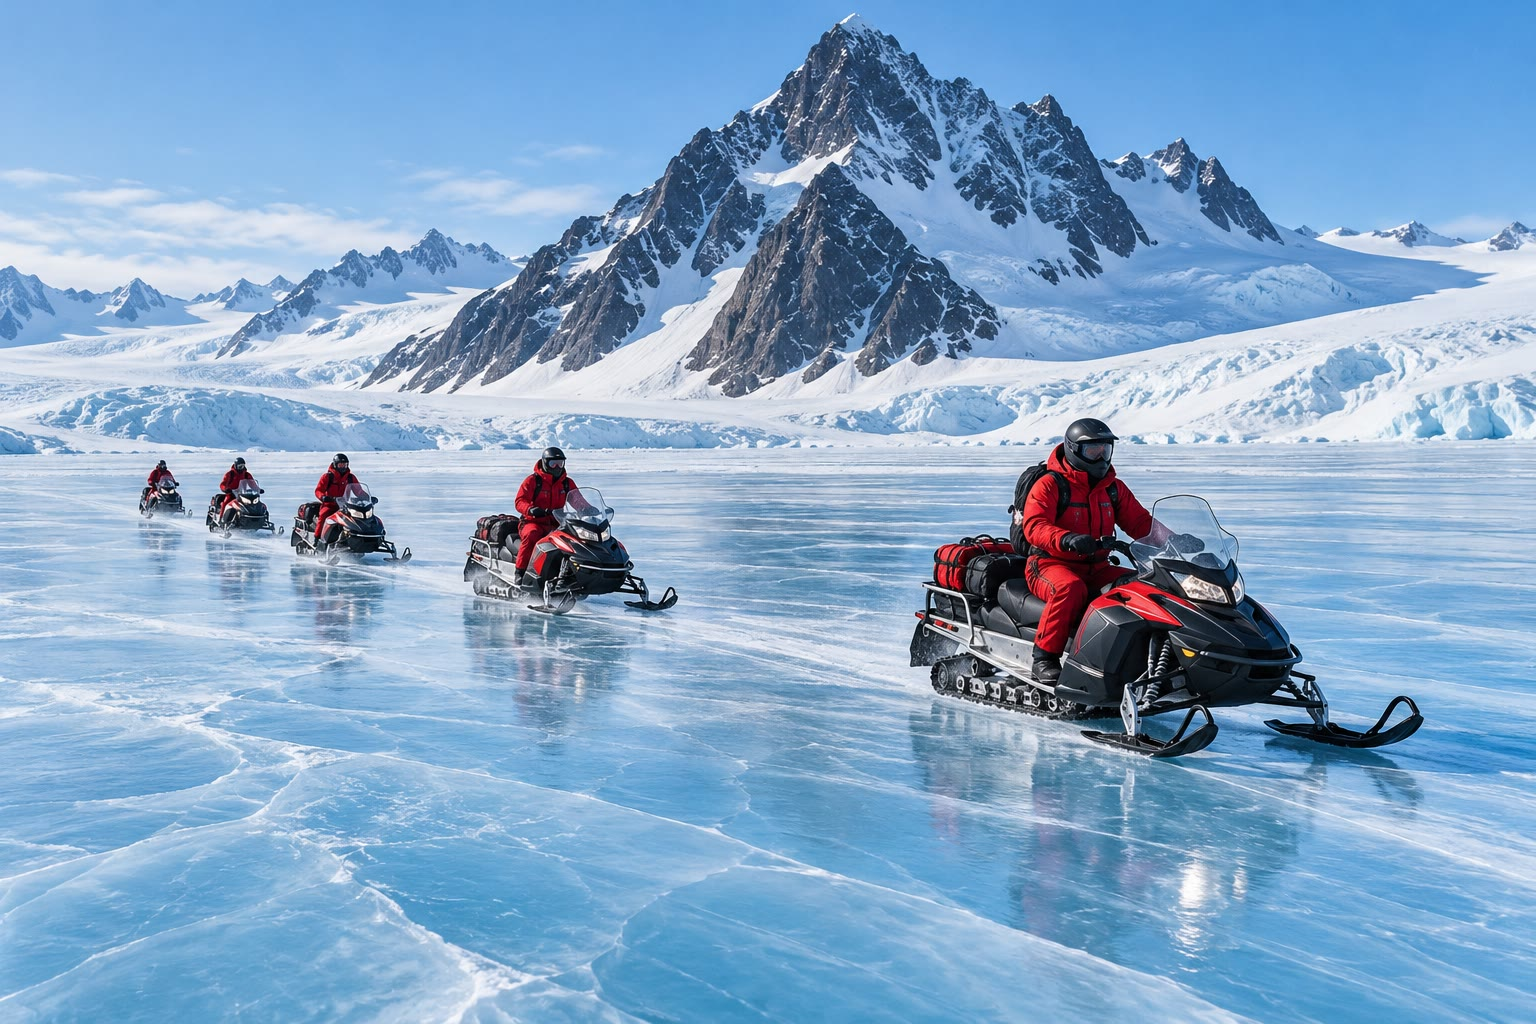
\includegraphics[width=\linewidth]{images/book4/ai/b2-blue-ice-search.jpg}

{\scriptsize चट्टानी शिखर के नीचे नीली बर्फ़ के एक क्षेत्र को पार करती, स्नोमोबाइलों पर
खोजकर्ताओं की एक पंक्ति (AI से बनाया गया चित्रण)।}
\end{minipage}
% ledger: folco06:blue-ice, data:b4-meteorites, nasa:antmet
\end{inthefield}

\subsection{कॉन्ड्राइट}

\begin{definition}[कॉन्ड्राइट, कार्बनमय कॉन्ड्राइट, कॉन्ड्रयूल, CAI]
\label{def:b2:planet-formation-meteorites:chondrule}
\emph{कॉन्ड्राइट}\index{कॉन्ड्राइट} वह पथरीला \omterm{def:b2:planet-formation-meteorites:fall-find}{उल्कापिंड} है जो
जुड़ने के बाद कभी नहीं पिघला, और जिसका संघटन, सबसे वाष्पशील
तत्त्वों को छोड़कर, सूर्य के संघटन के निकट है। उसका अधिकांश भाग
\emph{कॉन्ड्रयूलों}\index{कॉन्ड्रयूल} से बना है: सिलिकेट चट्टान की गोल बूँदें, जो एक मिलीमीटर के दसवें भाग से
लगभग एक सेंटीमीटर तक चौड़ी होती हैं और गलित से ठोस हुई हैं, और जो
लौह--निकल धातु और आयरन सल्फ़ाइड के कणों वाले एक महीन-कणीय आधात्री में जड़ी हैं। कुछ
कॉन्ड्राइटों में \emph{कैल्सियम--ऐलुमिनियम-समृद्ध अंतर्वेश}\index{कैल्सियम--ऐलुमिनियम-समृद्ध अंतर्वेश}
(CAI) होते हैं: कैल्सियम, ऐलुमिनियम
और टाइटेनियम के खनिजों के अनियमित सफ़ेद कण, जो नीहारिका के पहले संघनित हैं।
\emph{कार्बनमय कॉन्ड्राइट}\index{कार्बनमय कॉन्ड्राइट} वह कॉन्ड्राइट है जो
कार्बन, जलयुक्त खनिजों और आधात्री से समृद्ध हो, और जिसमें वाष्पशील
तत्त्वों की मात्रा सूर्य की मात्रा के सबसे निकट हो।
\end{definition}

\omterm{def:b2:planet-formation-meteorites:chondrule}{कॉन्ड्रयूल} केवल कुछ मिनट पिघले रहे और घंटों से दिनों में ठंडे
हुए: नीहारिका में किसी संक्षिप्त, स्थानीय, चमक-जैसे ऊष्मन ने, जिसका कारण अब भी
अज्ञात है, धूल के पुंजों को पिघलाया, जो बूँदों के रूप में जम गए, इससे पहले कि वे
धूल और धातु के साथ बटोरकर एक \omterm{def:b2:planet-formation-meteorites:planetesimal}{ग्रहाणु} में मिल जाते। वे सबसे
आदिम उल्कापिंडों के आयतन का \qty{90}{\percent} तक भरते हैं। CAI साधारण \omterm{def:b2:planet-formation-meteorites:chondrule}{कॉन्ड्राइटों} के
\qty{1}{\percent} से कम से लेकर कुछ \omterm{def:b2:planet-formation-meteorites:chondrule}{कार्बनमय कॉन्ड्राइटों} के \qty{10}{\percent} से अधिक तक होते हैं, और वे
एक-दूसरे के लगभग एक लाख वर्षों के भीतर बने।
% ledger: gail:meteorites, cy10:growth, cy10:chondrules, gail:chondrite-table, lugaro:cai

\begin{omfigure}
\begin{minipage}[c]{0.5\linewidth}
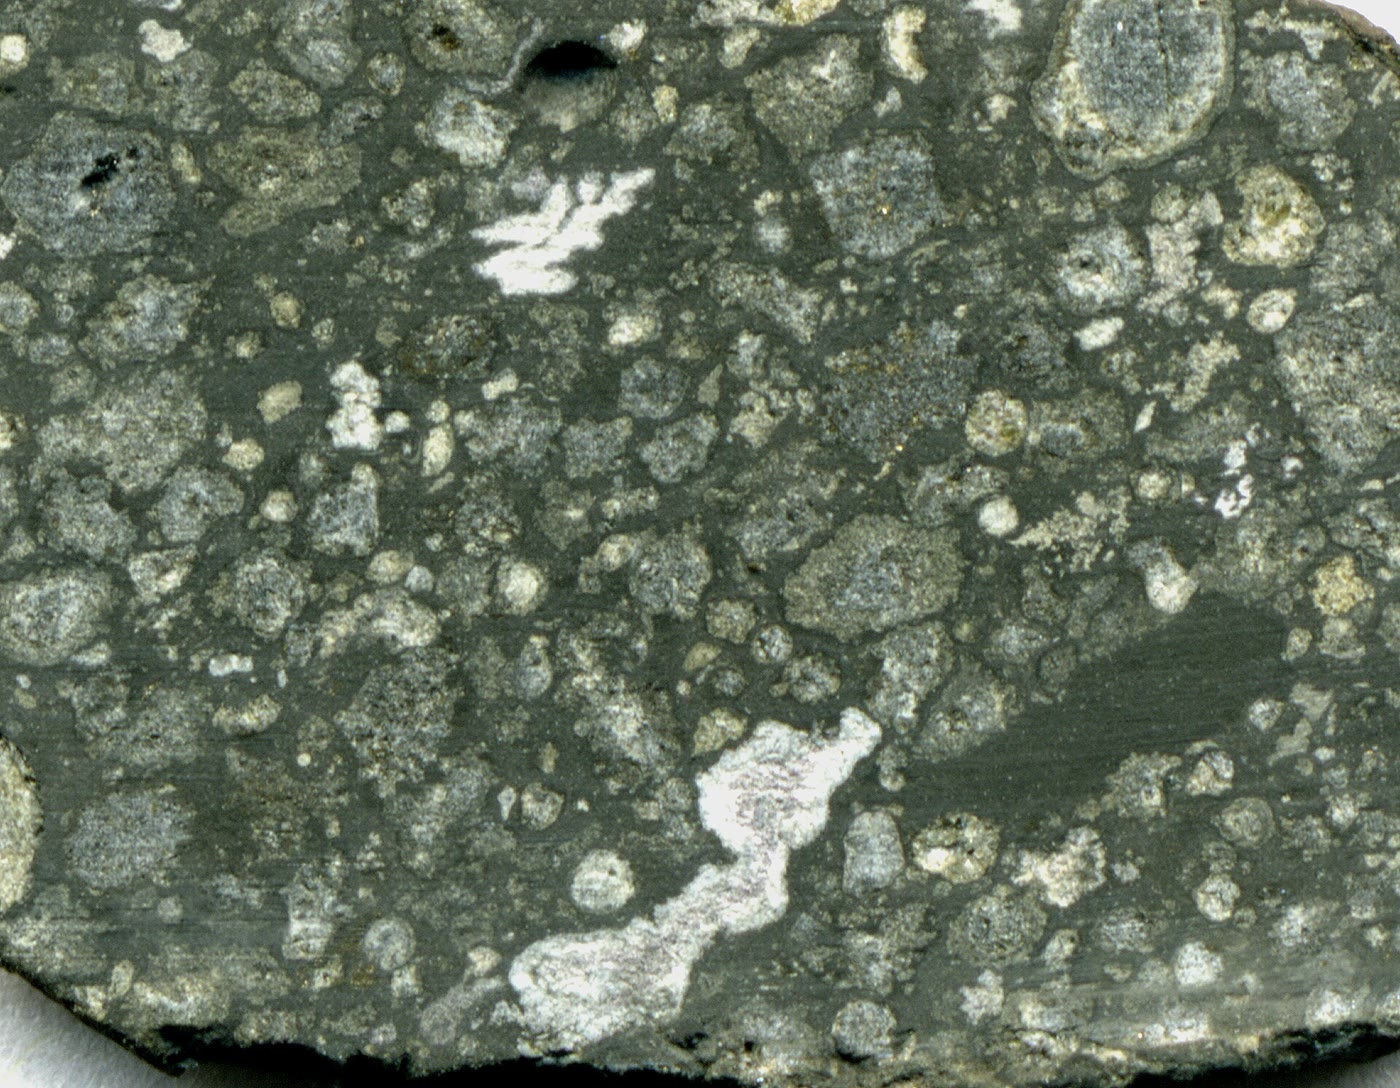
\includegraphics[width=\linewidth]{images/book4/b2-allende-chondrite.jpg}
\end{minipage}\hfill
\begin{minipage}[c]{0.46\linewidth}
{\small एलेंडे \omterm{def:b2:planet-formation-meteorites:chondrule}{कार्बनमय कॉन्ड्राइट} (वर्ग CV3) का कटा हुआ फलक, जो 1969 में
उत्तरी मेक्सिको में गिरा: लगभग दो टन एकत्र किए गए। गोल धूसर कण
\omterm{def:b2:planet-formation-meteorites:chondrule}{कॉन्ड्रयूल} हैं; अनियमित सफ़ेद धब्बे CAI हैं; गहरा सीमेंट आधात्री है।
दृश्य-क्षेत्र कुछ सेंटीमीटर चौड़ा है। फ़ोटो: James St.\ John, CC BY 2.0।}
\end{minipage}
% ledger: data:b4-meteorites, gail:chondrite-table
\end{omfigure}

\omterm{def:b2:planet-formation-meteorites:chondrule}{कॉन्ड्राइट} ऐसे समूहों में बँटते हैं जो अपने \omterm{def:b2:planet-formation-meteorites:chondrule}{कॉन्ड्रयूलों} के आकार और प्रचुरता, अपनी
धातु की मात्रा, अपने ओलिवीन की लौह-मात्रा और अपनी आधात्री के
अनुपात में भिन्न हैं (नीचे की तालिका)। साधारण \omterm{def:b2:planet-formation-meteorites:chondrule}{कॉन्ड्राइट} H, L और LL
में धातु और कुल लोहे की मात्रा उच्च, निम्न और अति निम्न होती है (परमाणु अनुपात
Fe/Si क्रमशः \num{0.80}, \num{0.59} और \num{0.53})।
% ledger: gail:chondrite-table

\begin{table}[h]
\centering
\small
\begin{tabular}{lcccccc}
\hline
 & H & L & LL & CI & CM & CV\\
\hline
\omterm{def:b2:planet-formation-meteorites:chondrule}{कॉन्ड्रयूल} (आयतन \%) & 60--80 & 60--80 & 60--80 & $\ll 1$ & 20 & 45\\
माध्य \omterm{def:b2:planet-formation-meteorites:chondrule}{कॉन्ड्रयूल} व्यास (mm) & 0.3 & 0.7 & 0.9 & --- & 0.3 & 1.0\\
CAI (आयतन \%) & 0.1--1 & 0.1--1 & 0.1--1 & $\ll 1$ & 5 & 10\\
आधात्री (आयतन \%) & 10--15 & 10--15 & 10--15 & $> 99$ & 70 & 40\\
लौह--निकल धातु (आयतन \%) & 10 & 5 & 2 & 0 & 0.1 & 0--5\\
ओलिवीन में फ़ेयालाइट (mol \%) & 16--20 & 23--26 & 27--32 & & & \\
\omterm{def:b2:planet-formation-meteorites:type}{शैलिकी प्रकार} & 3--6 & 3--6 & 3--6 & 1 & 2 & 3\\
उच्चतम तापमान (K) & 1220 & 1220 & 1220 & 430 & 670 & 870\\
\hline
\end{tabular}
\caption{साधारण (H, L, LL) और तीन \omterm{def:b2:planet-formation-meteorites:chondrule}{कार्बनमय कॉन्ड्राइट} समूहों के
गुण। फ़ेयालाइट: ओलिवीन का लौह अंत्य-सदस्य। डेटा: Gail और अन्य (2014)।}
\label{tab:b2:planet-formation-meteorites:chondrites}
% ledger: gail:chondrite-table
\end{table}

\begin{definition}[शैलिकी प्रकार]\label{def:b2:planet-formation-meteorites:type}
किसी \omterm{def:b2:planet-formation-meteorites:chondrule}{कॉन्ड्राइट} का \emph{शैलिकी प्रकार}\index{शैलिकी प्रकार} 1 से 6 तक की
वह संख्या है जो दर्ज करती है कि उसके जनक पिंड में उसके साथ क्या हुआ: प्रकार 3 सबसे
कम परिवर्तित है; प्रकार 4 से 6 उत्तरोत्तर अधिक गरम हुए हैं, उनके \omterm{def:b2:planet-formation-meteorites:chondrule}{कॉन्ड्रयूल} धुँधले
और उनके खनिज पुनःक्रिस्टलित तथा एकसमान संघटन के हैं; प्रकार 2 और 1
द्रव जल से उत्तरोत्तर अधिक परिवर्तित हैं, जिसने उनके खनिजों को मृत्तिकाओं में बदल दिया।
\end{definition}

तालिका की अंतिम पंक्ति हर समूह द्वारा प्राप्त उच्चतम तापमान देती है:
सबसे अधिक गरम हुए साधारण \omterm{def:b2:planet-formation-meteorites:chondrule}{कॉन्ड्राइटों} के लिए लगभग \qty{1220}{K} तक, CI \omterm{def:b2:planet-formation-meteorites:chondrule}{कॉन्ड्राइटों} के लिए
कभी \qty{430}{K} से अधिक नहीं, जो जल से तर रहे पर कभी गर्म नहीं हुए। यह
ऊष्मन, जैसा अंतिम अनुभाग दिखाता है, जनक पिंडों के भीतर से आया।
% ledger: gail:chondrite-table

\subsection{एकॉन्ड्राइट और लौह उल्कापिंड}

\begin{definition}[एकॉन्ड्राइट, लौह उल्कापिंड, पाषाण-लौह उल्कापिंड]
\label{def:b2:planet-formation-meteorites:classes}
\emph{एकॉन्ड्राइट}\index{एकॉन्ड्राइट} वह पथरीला \omterm{def:b2:planet-formation-meteorites:fall-find}{उल्कापिंड} है जो किसी पिघले पिंड में
गलित से क्रिस्टलित हुआ या उच्च तापमान पर पुनःक्रिस्टलित हुआ, और
इसलिए उसमें \omterm{def:b2:planet-formation-meteorites:chondrule}{कॉन्ड्रयूल} नहीं होते। \emph{लौह उल्कापिंड}\index{लौह उल्कापिंड}
मुख्यतः लौह--निकल धातु से बना होता है। \emph{पाषाण-लौह
उल्कापिंड}\index{पाषाण-लौह उल्कापिंड} लगभग बराबर मात्राओं में धातु और सिलिकेट से
बना होता है।
\end{definition}

ये उन पिंडों के टुकड़े हैं जो पिघले और पृथक हुए: \omterm{def:b2:planet-formation-meteorites:classes}{एकॉन्ड्राइट} उनकी
भूपर्पटियाँ और प्रावार हैं, \omterm{def:b2:planet-formation-meteorites:classes}{लौह उल्कापिंड} उनके धात्विक क्रोड, और \omterm{def:b2:planet-formation-meteorites:classes}{पाषाण-लौह उल्कापिंड} वहाँ से आते हैं जहाँ
धातु और सिलिकेट मिलते थे। \omterm{def:b2:planet-formation-meteorites:classes}{एकॉन्ड्राइटों} का सबसे बड़ा परिवार, हॉवर्डाइट,
यूक्राइट और डायोजेनाइट (HED), जो बेसाल्ट और पाइरॉक्सीन-समृद्ध चट्टानें हैं, सभी पतित
उल्कापिंडों का \qty{5.5}{\percent} है। उसके स्रोत का पता, उसके स्पेक्ट्रम और
उसकी कक्षा से, लगभग \qty{525}{km} चौड़े क्षुद्रग्रह वेस्टा तक लगाया गया, और डॉन
अंतरिक्ष-यान ने, जो 2011 में वेस्टा पहुँचा, इसकी पुष्टि की: वेस्टा के पृष्ठ का रसायन
और खनिज-संघटन HED उल्कापिंडों से मेल खाता है, उसके दक्षिणी ध्रुव के निकट
\qty{500}{km} चौड़ी एक द्रोणी दिखाती है कि टुकड़े कहाँ से उखड़े,
और उसका गुरुत्व-क्षेत्र लगभग \qty{225}{km} चौड़े लौह क्रोड की ओर संकेत करता है।
वेस्टा अपने इतिहास के आरंभ में लगभग या पूरी तरह पिघला था। अन्य \omterm{def:b2:planet-formation-meteorites:classes}{एकॉन्ड्राइट}
चंद्रमा और मंगल से आते हैं। संग्रहों के \omterm{def:b2:planet-formation-meteorites:fall-find}{उल्कापिंड} लगभग सौ भिन्न
जनक पिंडों से आए प्रतीत होते हैं।
% ledger: data:b4-meteorites, nasa:vesta-dawn, gail:meteorites

\omterm{def:b2:planet-formation-meteorites:classes}{लौह उल्कापिंड} इस बात का अभिलेख रखते हैं कि उनके क्रोड कैसे ठंडे हुए। काटकर
अम्ल से निक्षारित फलक पर पट्टिकाओं का एक जालीदार प्रतिरूप दिखता है (नीचे का चित्र): उच्च
तापमान पर धातु लोहे और निकल की एक ही मिश्रधातु होती है; धीरे ठंडा होने पर
निकल-निर्धन मिश्रधातु मूल क्रिस्टल के तलों के अनुदिश पट्टिकाओं में बढ़ती है,
और शीतलन जितना धीमा, पट्टिकाएँ उतनी चौड़ी। अनेक \omterm{def:b2:planet-formation-meteorites:classes}{लौह उल्कापिंडों} पर मापी गई
पट्टिका-चौड़ाइयाँ उन क्रोडों की शीतलन-दरें देती हैं जिनसे वे आए।
% ledger: gail:meteorites

\begin{omfigure}
\begin{minipage}[c]{0.5\linewidth}
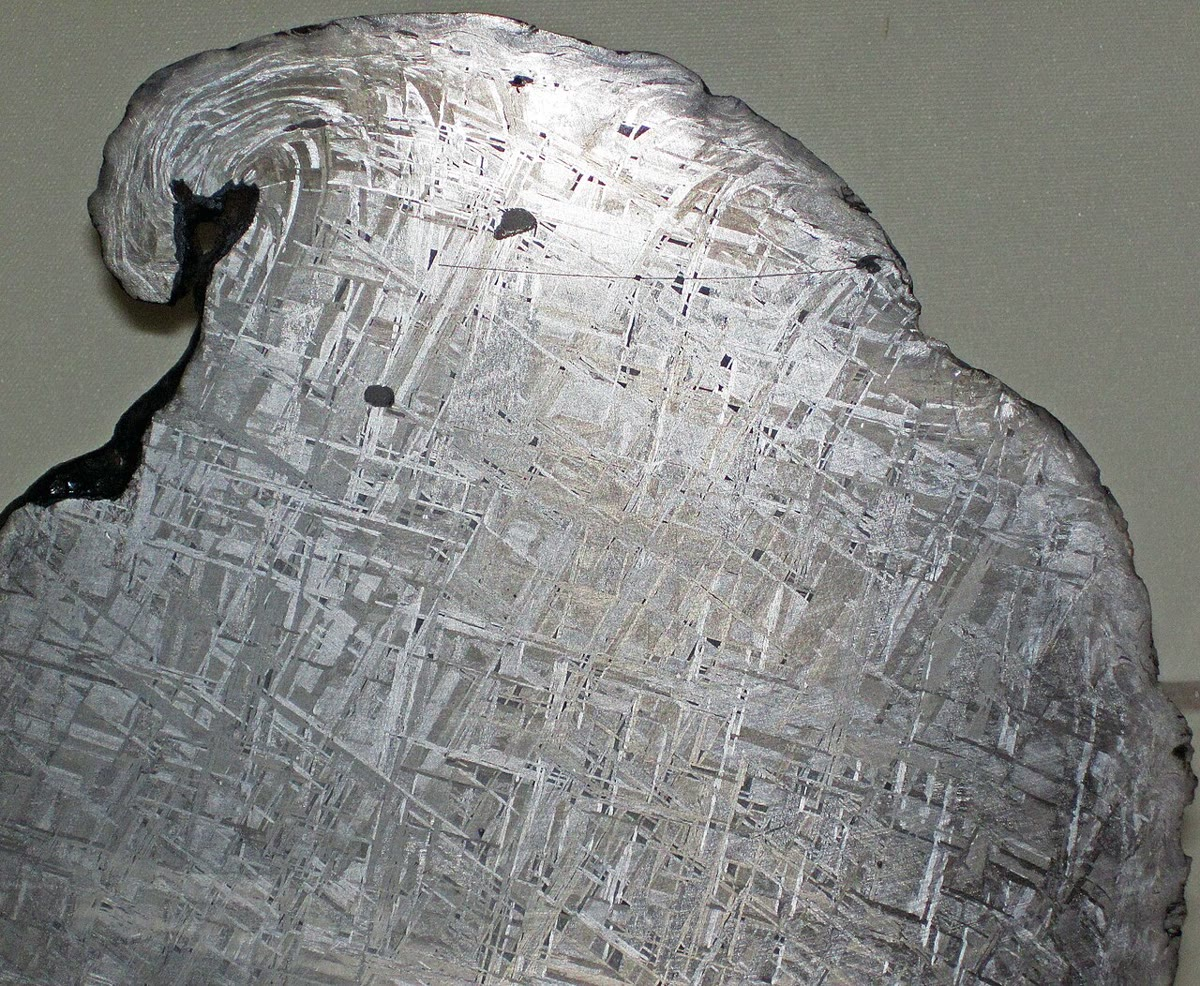
\includegraphics[width=\linewidth]{images/book4/b2-gibeon-widmanstatten.jpg}
\end{minipage}\hfill
\begin{minipage}[c]{0.46\linewidth}
{\small नामीबिया में मिले गिबियन \omterm{def:b2:planet-formation-meteorites:classes}{लौह उल्कापिंड} के एक टुकड़े का कटा, चमकाया और
अम्ल से निक्षारित फलक: लौह--निकल मिश्रधातु की पट्टिकाओं का जालीदार प्रतिरूप (विडमनश्टेटन
प्रतिरूप) तब बढ़ा जब उसके जनक पिंड का धात्विक क्रोड धीरे-धीरे ठंडा हुआ। फ़ोटो: James St.\ John,
CC BY 2.0।}
\end{minipage}
% ledger: data:b4-meteorites
\end{omfigure}

\section{सौरमंडल का आयु-निर्धारण}

सौरमंडल की आयु उसके सबसे पुराने ठोसों की आयु है। CAI की यूरेनियम--सीसा
समकालरेखाएँ, पुस्तक 3 (स्नातक वर्ष 1) की भाँति बनाई गई, \qtyrange{4567}{4568}{\Ma} देती हैं;
CAI एक-दूसरे के लगभग \qty{0.1}{Myr} के भीतर बने, यह समय इतना छोटा है
कि उनकी आयु को सूर्य का जन्म माना जा सके। अगले
कुछ मिलियन वर्षों की घटनाओं, अर्थात् \omterm{def:b2:planet-formation-meteorites:chondrule}{कॉन्ड्रयूलों} के निर्माण और प्रथम पिंडों के जुड़ने और
पिघलने, की आयु CAI के सापेक्ष सबसे अच्छी तरह आँकी जाती है, उन घड़ियों से
जो तेज़ चलीं और जल्दी रुक गईं।
% ledger: lugaro:cai

\begin{definition}[अल्पजीवी रेडियोनाभिक]
\label{def:b2:planet-formation-meteorites:slr}
\emph{अल्पजीवी रेडियोनाभिक}\index{अल्पजीवी रेडियोनाभिक} वह
रेडियोधर्मी नाभिक है जिसकी अर्ध-आयु लगभग \num{0.1} से \qty{100}{Myr} हो,
जो सौरमंडल के बनते समय उपस्थित था और अब विलुप्त है, और जिसकी पूर्व उपस्थिति
उन खनिजों में उसकी संतति के आधिक्य से दिखती है जो उसके तत्त्व से
समृद्ध थे।
\end{definition}

सबसे प्रसिद्ध ऐलुमिनियम-26 है। यह \qty{0.717}{Myr} की अर्ध-आयु से मैग्नीशियम-26 में
क्षय होता है (इसकी माध्य आयु \qty{1.035}{Myr} है)। जब CAI बने, तब लगभग \num{19000} में से
एक ऐलुमिनियम परमाणु ऐलुमिनियम-26 था: अनुपात $\ce{^{26}Al}/\ce{^{27}Al}$ का
मान $(5.23 \pm 0.13)\times10^{-5}$ था, जो
\emph{मानक} मान है। अन्य अल्पजीवी नाभिक अधिक लंबी अवधियाँ ढँकते हैं (नीचे की
तालिका)।
% ledger: lugaro:al26, lugaro:slr-table

\begin{table}[h]
\centering
\small
\begin{tabular}{lllcc}
\hline
नाभिक & संतति & संदर्भ & अर्ध-आयु (\unit{Myr}) & आरंभिक अनुपात\\
\hline
\ce{^{26}Al} & \ce{^{26}Mg} & \ce{^{27}Al} & 0.717 & $5.23\times10^{-5}$\\
\ce{^{60}Fe} & \ce{^{60}Ni} & \ce{^{56}Fe} & 2.62 & $1.0\times10^{-8}$\\
\ce{^{53}Mn} & \ce{^{53}Cr} & \ce{^{55}Mn} & 3.74 & $7\times10^{-6}$\\
\ce{^{107}Pd} & \ce{^{107}Ag} & \ce{^{108}Pd} & 6.5 & $6.6\times10^{-5}$\\
\ce{^{182}Hf} & \ce{^{182}W} & \ce{^{180}Hf} & 8.90 & $1.02\times10^{-4}$\\
\ce{^{129}I} & \ce{^{129}Xe} & \ce{^{127}I} & 15.7 & $1.28\times10^{-4}$\\
\hline
\end{tabular}
\caption{प्रारंभिक सौरमंडल के कुछ \omterm{def:b2:planet-formation-meteorites:slr}{अल्पजीवी रेडियोनाभिक}, उनकी स्थायी
संतति, उसी तत्त्व का वह स्थायी समस्थानिक जो संदर्भ के रूप में प्रयुक्त है, उनकी
अर्ध-आयु और CAI के बनते समय संदर्भ से उनका अनुपात। डेटा: Lugaro और
अन्य (2018)।}
\label{tab:b2:planet-formation-meteorites:slr}
% ledger: lugaro:al26, lugaro:slr-table
\end{table}

\begin{proposition}[विलुप्त नाभिक से सापेक्ष आयु]
\label{prop:b2:planet-formation-meteorites:relative-age}
यदि CAI के बनते समय किसी अल्पजीवी नाभिक का अपने संदर्भ समस्थानिक से अनुपात
हर जगह $R_0$ था, और किसी वस्तु में उसके बनते समय वह $R$ पाया जाता है,
तो वह वस्तु
\[
  \Delta t = \tau \ln\frac{R_0}{R}
\]
CAI के बाद बनी, जहाँ $\tau$ नाभिक की माध्य आयु है। $\delta R$ की त्रुटि यदि $R$ पर हो,
तो उससे $\tau\,\delta R/R$ की त्रुटि आती है, जो $\Delta t$ पर होती है।
\end{proposition}

\begin{proof}
संदर्भ समस्थानिक स्थायी है, इसलिए अनुपात स्वयं रेडियोधर्मी
नाभिक की भाँति क्षय होता है: $R = R_0 e^{-\Delta t/\tau}$। लघुगणक लेने पर
$\Delta t = \tau\ln(R_0/R)$। अवकलन करने पर $\mathrm d(\Delta t) =
-\tau\,\mathrm dR/R$।
\end{proof}

इस प्रकार अनुपात पर \qty{10}{\percent} की सापेक्ष त्रुटि की कीमत ऐलुमिनियम-26 के साथ
\qty{0.1}{Myr} है, पर मैंगनीज़-53 के साथ \qty{0.54}{Myr} और
हैफ़नियम-182 के साथ \qty{1.3}{Myr}: हर घड़ी केवल अपनी कुछ
माध्य आयुओं तक ही सटीक है, और सही घड़ी घटना पर निर्भर करती है। किसी
वस्तु में अनुपात $R$ उसके खनिजों से पढ़ा जाता है।
% ledger: lugaro:al26, lugaro:slr-table

\begin{proposition}[ऐलुमिनियम--मैग्नीशियम समकालरेखा]
\label{prop:b2:planet-formation-meteorites:al-mg}
मान लीजिए किसी एक वस्तु के कई खनिज समय $\Delta t$ पर साथ-साथ बनते हैं, मैग्नीशियम की
समान समस्थानिक संरचना $(\ce{^{26}Mg}/\ce{^{24}Mg})_0$ के साथ, पर
भिन्न अनुपातों $\ce{^{27}Al}/\ce{^{24}Mg}$ के साथ, और तब से बंद रहते हैं। आज वे
इस सरल रेखा पर स्थित हैं:
\[
  \frac{\ce{^{26}Mg}}{\ce{^{24}Mg}}
  = \left(\frac{\ce{^{26}Mg}}{\ce{^{24}Mg}}\right)_0
  + R\,\frac{\ce{^{27}Al}}{\ce{^{24}Mg}},
\]
जिसकी प्रवणता वस्तु के बनते समय का अनुपात $R = \ce{^{26}Al}/\ce{^{27}Al}$
है।
\end{proposition}

\begin{proof}
निर्माण के समय उपस्थित हर ऐलुमिनियम-26 परमाणु तब से
मैग्नीशियम-26 परमाणु बन चुका है, इसलिए किसी खनिज ने
$\ce{^{26}Al}_{\text{तब}} = R\,\ce{^{27}Al}$ मैग्नीशियम-26 परमाणु प्राप्त किए, क्योंकि ऐलुमिनियम-27
स्थायी है। मैग्नीशियम-24 परमाणुओं की संख्या से, जो अपरिवर्तित है, भाग देने पर
रेखा मिलती है।
\end{proof}

प्लेजियोक्लेज़ जैसे ऐलुमिनियम-समृद्ध, मैग्नीशियम-निर्धन खनिज
मैग्नीशियम-26 का बड़ा आधिक्य दिखाते हैं; ओलिवीन, जो लगभग ऐलुमिनियम-रहित है, कोई नहीं। इसी प्रकार
प्रारंभिक सौरमंडल का कालक्रम बनाया गया: पहले CAI; फिर अगले कुछ मिलियन वर्षों में
\omterm{def:b2:planet-formation-meteorites:chondrule}{कॉन्ड्रयूल}, और \omterm{def:b2:planet-formation-meteorites:chondrule}{कॉन्ड्रयूलों} के साक्ष्य गैस-चक्रिका की
आयु को पाँच मिलियन वर्ष से कम रखते हैं; \omterm{def:b2:planet-formation-meteorites:chondrule}{कॉन्ड्राइटों}
के जनक पिंड अपने सबसे युवा \omterm{def:b2:planet-formation-meteorites:chondrule}{कॉन्ड्रयूलों} के बाद जुड़े।
डायोजेनाइट, जो वेस्टा के प्रावार की चट्टानें हैं, CAI के लगभग दस लाख वर्षों के भीतर
क्रिस्टलित होने लगे, और वेस्टा का क्रोड पहले एक से
चार मिलियन वर्षों के भीतर बना: \omterm{def:b2:planet-formation-meteorites:classes}{लौह उल्कापिंड} और \omterm{def:b2:planet-formation-meteorites:classes}{एकॉन्ड्राइट} कई
\omterm{def:b2:planet-formation-meteorites:chondrule}{कॉन्ड्राइटों} से पुराने हैं।
% ledger: lugaro:cai, gail:vesta, gail:meteorites

\section{ऐलुमिनियम-26 से ऊष्मा और प्रथम गलन}

जिस ऊष्मा ने वेस्टा को पिघलाया, और साधारण \omterm{def:b2:planet-formation-meteorites:chondrule}{कॉन्ड्राइटों} को कायांतरित किया, वह
कहाँ से आई? मॉडल और \omterm{def:b2:planet-formation-meteorites:fall-find}{उल्कापिंड} सहमत हैं कि सबसे प्रारंभिक पिंडों में
प्रमुख स्रोत ऐलुमिनियम-26 का क्षय था। कॉन्ड्राइटी संघटन की चट्टान में वह आरंभ में
प्रति किलोग्राम \qty{5}{MJ} लिए हुए था, जो कुछ मिलियन वर्षों में मुक्त होने को तैयार थी:
यदि ऊष्मा बाहर न निकल पाती, तो चट्टान को हज़ारों केल्विन गरम करने के लिए पर्याप्त।
% ledger: lugaro:heat, lugaro:melting

\begin{proposition}[ऐलुमिनियम-26 द्वारा ग्रहाणु का ऊष्मन]
\label{prop:b2:planet-formation-meteorites:heating}
जो चट्टान प्रति किलोग्राम रेडियोधर्मी शक्ति $H_0 e^{-t/\tau}$ प्राप्त करती है,
विशिष्ट ऊष्मा-धारिता $c$ रखती है और कोई ऊष्मा नहीं खोती, वह समय $t_a$ पर अपनी अभिवृद्धि के
बाद इस प्रकार गरम होती है:
\[
  T(t) = T_0 + \frac{H_0\tau}{c}\left(e^{-t_a/\tau} - e^{-t/\tau}\right),
\]
और शिखर तापमान
$T_{\max} = T_0 + (H_0\tau/c)\,e^{-t_a/\tau}$ की ओर प्रवृत्त होती है। क्रांतिक तापमान
$T_c > T_0$ तभी प्राप्त होता है जब पिंड की अभिवृद्धि इससे पहले हुई हो:
\[
  t_a^* = \tau\ln\frac{H_0\tau}{c\,(T_c - T_0)}.
\]
\end{proposition}

\begin{proof}
बिना हानि के $c\,\mathrm dT/\mathrm dt = H_0 e^{-t/\tau}$। इसका
$t_a$ से, जहाँ $T = T_0$ है, समाकलन करने पर
$c\,(T - T_0) = H_0\tau\,(e^{-t_a/\tau} - e^{-t/\tau})$ मिलता है, जो $H_0\tau e^{-t_a/\tau}$
की ओर प्रवृत्त होता है जब $t \to \infty$। $T_{\max} = T_c$ रखकर
$t_a$ के लिए हल करने पर $t_a^*$ मिलता है; पहले की अभिवृद्धि के लिए शिखर अधिक ऊँचा है।
\end{proof}

साधारण \omterm{def:b2:planet-formation-meteorites:chondrule}{कॉन्ड्राइटों} के जनक पिंड का एक मॉडल
$H_0 = \qty{1.9e-7}{W.kg^{-1}}$, $c = \qty{837}{J.kg^{-1}.K^{-1}}$ और
$T_0 = \qty{250}{K}$ लेता है। तब $H_0\tau/c$ लगभग \qty{7400}{K} है। तीन
तापमान महत्त्वपूर्ण हैं: \qty{750}{K} के निकट सरंध्र चट्टान सिंटरित होकर
संहत होने लगती है; \qty{1200}{K} के निकट धातु और आयरन सल्फ़ाइड साथ-साथ पिघलने
लगते हैं; \qty{1700}{K} के निकट अंतिम सिलिकेट पिघलते हैं। जिस पिंड की अभिवृद्धि
\qty{1.7}{Myr} से पहले हुई वह पूरी तरह पिघला; \qty{2.1}{Myr} से पहले उसकी धातु और सल्फ़ाइड
पिघले और एक क्रोड में डूब सके; लगभग \qty{2.8}{Myr} तक वह कम से कम
सिंटरित और कायांतरित हुआ; बाद के पिंड ठंडे रहे (नीचे का चित्र)।
% ledger: gail:params, gail:temps, lugaro:al26

\begin{omfigure}
\begin{tikzpicture}
\begin{axis}[omrecord, name=left, width=0.45\linewidth, height=6.0cm,
  xmin=0, xmax=8, ymin=0, ymax=2300,
  xlabel={CAI के बाद का समय (\unit{Myr})}, ylabel={तापमान (K)},
  tick label style={font=\scriptsize}, label style={font=\small}]
\addplot[black!45, densely dashed, domain=0:8, samples=2] {750};
\addplot[black!45, densely dashed, domain=0:8, samples=2] {1200};
\addplot[black!45, densely dashed, domain=0:8, samples=2] {1700};
\addplot[thick, red!75!black] table[x=t_Myr, y=T_K] {figdata/out/bachelor-2-al26-ta15.dat};
\addplot[thick, orange!80!black] table[x=t_Myr, y=T_K] {figdata/out/bachelor-2-al26-ta20.dat};
\addplot[thick, teal!70!black] table[x=t_Myr, y=T_K] {figdata/out/bachelor-2-al26-ta25.dat};
\addplot[thick, blue!70!black] table[x=t_Myr, y=T_K] {figdata/out/bachelor-2-al26-ta30.dat};
\node[font=\tiny, red!75!black, anchor=south east] at (axis cs:7.9,1995) {$t_a = \qty{1.5}{Myr}$};
\node[font=\tiny, orange!80!black, anchor=south east] at (axis cs:7.9,1325) {2};
\node[font=\tiny, teal!70!black, anchor=south east] at (axis cs:7.9,915) {2.5};
\node[font=\tiny, blue!70!black, anchor=north east] at (axis cs:7.9,650) {3};
\node[font=\tiny, black!60, anchor=south west] at (axis cs:0.1,1700) {सिलिकेट पिघले};
\node[font=\tiny, black!60, anchor=south west] at (axis cs:0.1,1200) {\shortstack[l]{धातु-सल्फ़ाइड\\गलन}};
\node[font=\tiny, black!60, anchor=south west] at (axis cs:0.1,750) {सिंटरण};
\end{axis}
\begin{axis}[omrecord, at={(left.east)}, anchor=west, xshift=2.1cm, width=0.45\linewidth,
  height=6.0cm, xmin=0, xmax=4, ymin=0, ymax=8000,
  xlabel={अभिवृद्धि-समय $t_a$ (\unit{Myr})}, ylabel={शिखर तापमान (K)},
  tick label style={font=\scriptsize}, label style={font=\small},
  scaled y ticks=false, yticklabel style={/pgf/number format/1000 sep={\,}}]
\addplot[black!45, densely dashed, domain=0:4, samples=2] {750};
\addplot[black!45, densely dashed, domain=0:4, samples=2] {1200};
\addplot[black!45, densely dashed, domain=0:4, samples=2] {1700};
\addplot[thick, black] table[x=ta_Myr, y=Tpeak_K] {figdata/out/bachelor-2-al26-peak.dat};
\draw[black!60] (axis cs:1.69,0) -- (axis cs:1.69,1700);
\draw[black!60] (axis cs:2.13,0) -- (axis cs:2.13,1200);
\node[font=\tiny, black!70, anchor=south] at (axis cs:2.0,4500) {\qty{1.7}{Myr}};
\draw[black!50, -latex] (axis cs:2.0,4450) -- (axis cs:1.71,1800);
\node[font=\tiny, black!70, anchor=south] at (axis cs:2.9,3300) {\qty{2.1}{Myr}};
\draw[black!50, -latex] (axis cs:2.9,3250) -- (axis cs:2.16,1300);
\end{axis}
\end{tikzpicture}

\par\smallskip{\small बिना ऊष्मा-हानि वाले कॉन्ड्राइटी पिंड के भीतरी भाग का ऐलुमिनियम-26 द्वारा
ऊष्मन (ऊपर की प्रतिज्ञप्ति; $H_0 = \qty{1.9e-7}{W.kg^{-1}}$,
$c = \qty{837}{J.kg^{-1}.K^{-1}}$, $T_0 = \qty{250}{K}$, $\tau = \qty{1.035}{Myr}$)।
बाएँ: CAI के 1.5, 2, 2.5 और \qty{3}{Myr} बाद अभिवृद्ध पिंडों के लिए
समय के सापेक्ष तापमान। दाएँ: अभिवृद्धि-समय के सापेक्ष शिखर तापमान; जो पिंड
\qty{1.7}{Myr} से पहले अभिवृद्ध हुए वे पिघले, \qty{2.1}{Myr} से पहले वालों की धातु और सल्फ़ाइड पिघले।
वास्तविक पिंड ऊष्मा का कुछ भाग गलन पर खर्च करते हैं, जो तापमान को सीमित करता है, और
अपने पृष्ठ के निकट ऊष्मा खोते हैं। मॉडल-मान: Gail और अन्य (2014)।}
% ledger: gail:params, gail:temps, lugaro:al26
\end{omfigure}

प्रतिज्ञप्ति ऊष्मा-हानि की उपेक्षा करती है, जो केवल किसी बड़े पिंड के गहरे भीतर ही मान्य है।
ऊष्मा $\sqrt{\kappa t}$ की दूरी तक, समय $t$ में, विसरित होती है, जहाँ
$\kappa$ चट्टान की तापीय विसरणशीलता है: मॉडल के मानों से,
ऐलुमिनियम-26 की एक माध्य आयु में लगभग \qty{5}{km} (\cref{exo:b2:planet-formation-meteorites:12})। इससे बहुत
छोटे पिंड अपनी ऊष्मा उतनी ही तेज़ी से खोते हैं जितनी तेज़ी से बनाते हैं; विस्तृत मॉडल दिखाते हैं
कि \qtyrange{10}{20}{km} से अधिक चौड़े पिंड पिघल सकते थे।
% ledger: gail:params, lugaro:melting

\begin{definition}[ग्रहीय विभेदन]
\label{def:b2:planet-formation-meteorites:differentiation}
\emph{ग्रहीय विभेदन}\index{ग्रहीय विभेदन} किसी पिंड का, एक बार
पिघलने या आंशिक रूप से पिघलने पर, भिन्न संघटन और घनत्व की परतों में पृथक्करण है:
एक धात्विक क्रोड, एक सिलिकेट प्रावार और अंतिम गलितों से बनी
एक भूपर्पटी।
\end{definition}

इस प्रकार \omterm{def:b2:planet-formation-meteorites:fall-find}{उल्कापिंड} दो प्रकार के आरंभिक पिंडों का अभिलेख रखते हैं। जो लगभग पहले दो
मिलियन वर्षों के भीतर बने, उनमें पिघलने और विभेदित होने के लिए पर्याप्त ऐलुमिनियम-26
था: उनके क्रोड \omterm{def:b2:planet-formation-meteorites:classes}{लौह उल्कापिंड} हैं, उनकी भूपर्पटियाँ और प्रावार
\omterm{def:b2:planet-formation-meteorites:classes}{एकॉन्ड्राइट}, और वेस्टा उत्तरजीवी है। जो बाद में बने वे \omterm{def:b2:planet-formation-meteorites:chondrule}{कॉन्ड्राइट} ही
रहे, भीतर से उतने गरम हुए जितना उनकी जन्म-तिथि और हर टुकड़े की
गहराई तय करती थी: सबसे गहरे प्रकार 6 बने, सबसे उथले प्रकार 3 ही
रहे। स्वयं पृथ्वी, जो दोनों प्रकार के भ्रूणों और \omterm{def:b2:planet-formation-meteorites:planetesimal}{ग्रहाणुओं} से बनी और
महा-संघट्टों से टकराई, अपने क्रोड, प्रावार और भूपर्पटी में विभेदित हुई।
% ledger: gail:meteorites, gail:vesta, gail:temps

\section{अभ्यास}

\begin{exercise}[$\star$]\label{exo:b2:planet-formation-meteorites:1}
न्यूनतम द्रव्यमान \omterm{def:b2:planet-formation-meteorites:nebula}{सौर नीहारिका} में, गैस का पृष्ठ-घनत्व
\qty{1}{au} और \qty{5.2}{au} पर, तथा ठोसों का पृष्ठ-घनत्व
\qty{1}{au} पर (केवल चट्टान, $Z_{\mathrm{rel}} = 0.33$) और \qty{5.2}{au} पर (सभी बर्फ़ें
संघनित, $Z_{\mathrm{rel}} = 1$) परिकलित कीजिए। \qty{5.2}{au} पर गैस ठोसों से कितने
गुना भारी है?
% ledger: cy10:mmsn
\end{exercise}

\begin{exercise}[$\star$]\label{exo:b2:planet-formation-meteorites:2}
\omterm{def:b2:planet-formation-meteorites:condensation}{संघनन तापमानों} वाले चित्र की सहायता से ऐलुमिनियम, सोडियम,
मैग्नीशियम, लोहा, सल्फ़र और ऑक्सीजन (जल-बर्फ़ के रूप में) को पहले संघनित होने वाले से
अंतिम तक क्रम में रखिए, और हर एक का वाष्पशीलता-समूह बताइए। आप इनमें से किन्हें
CAI में समृद्ध पाने की, और किन्हें सूर्य की तुलना में पृथ्वी में न्यून पाने की अपेक्षा करेंगे?
% ledger: lodders:tc-table, lodders:groups
\end{exercise}

\begin{exercise}[$\star$]\label{exo:b2:planet-formation-meteorites:3}
सूची में \num{1107} \omterm{def:b2:planet-formation-meteorites:fall-find}{पतित उल्कापिंड} हैं, जिनमें 856 साधारण \omterm{def:b2:planet-formation-meteorites:chondrule}{कॉन्ड्राइट} और
49 लौह हैं, और \num{44534} \omterm{def:b2:planet-formation-meteorites:fall-find}{प्राप्त उल्कापिंड}, जिनमें \num{38647} साधारण \omterm{def:b2:planet-formation-meteorites:chondrule}{कॉन्ड्राइट},
\num{1020} लौह हैं और \num{22096} \ang{60} दक्षिणी अक्षांश के दक्षिण से आते हैं। पतित और
प्राप्त उल्कापिंडों में साधारण \omterm{def:b2:planet-formation-meteorites:chondrule}{कॉन्ड्राइटों} और \omterm{def:b2:planet-formation-meteorites:classes}{लौह उल्कापिंडों} का अंश, तथा अंटार्कटिक
प्राप्त उल्कापिंडों का अंश परिकलित कीजिए। वर्ग किन अनुपातों में पृथ्वी पर पहुँचते हैं, इसका अनुमान लगाने के लिए
आप किस नमूने का प्रयोग करेंगे, और क्यों?
% ledger: data:b4-meteorites
\end{exercise}

\begin{exercise}[$\star$]\label{exo:b2:planet-formation-meteorites:4}
किसी वस्तु के खनिज आरंभिक अनुपात
$\ce{^{26}Al}/\ce{^{27}Al} = \num{1.0e-5}$ देते हैं। वह CAI के कितने समय बाद बनी?
$R_0 = \num{5.23e-5}$ और माध्य आयु \qty{1.035}{Myr} लीजिए।
% ledger: lugaro:al26
\end{exercise}

\begin{exercise}[$\star\star$]\label{exo:b2:planet-formation-meteorites:5}
\cref{prop:b2:planet-formation-meteorites:disc-mass} का प्रयोग करके,
\qty{1}{au} पर $\Sigma_1 = \qty{2.2e4}{kg.m^{-2}}$ लेकर (\qty{1}{au} $=
\qty{1.496e11}{m}$, $M_\odot = \qty{1.989e30}{kg}$), \qty{30}{au} के भीतर और \qty{100}{au} के भीतर
न्यूनतम द्रव्यमान नीहारिका का द्रव्यमान सौर द्रव्यमानों में परिकलित कीजिए।
प्रेक्षित चक्रिकाओं, \numrange{0.001}{0.1} सौर द्रव्यमान, से तुलना कीजिए।
% ledger: cy10:mmsn
\end{exercise}

\begin{exercise}[$\star\star$]\label{exo:b2:planet-formation-meteorites:6}
निष्क्रिय चक्रिका $T = \qty{120}{K}\,(r/\qty{1}{au})^{-3/7}$ में, ज्ञात कीजिए कि जल-बर्फ़
(\qty{182}{K}) और मीथेन-बर्फ़ (\qty{41}{K}) कहाँ स्थायी होती हैं। सीधी
धूप में एक कण \qty{2.3}{au} पर \qty{182}{K} तक पहुँचता है। \omterm{def:b2:planet-formation-meteorites:snow-line}{हिम रेखा} के दो अनुमान
भिन्न क्यों हैं, और ग्रहों को बनाने वाले पिंडों पर कौन-सा लागू होता है?
% ledger: cy10:passive, lodders:phases
\end{exercise}

\begin{exercise}[$\star\star$]\label{exo:b2:planet-formation-meteorites:7}
$b = 5$ के साथ, न्यूनतम द्रव्यमान नीहारिका में \qty{1}{au} पर किसी भ्रूण का विलगन द्रव्यमान
($\Sigma_p = \qty{10.9}{g.cm^{-2}}$), और \omterm{def:b2:planet-formation-meteorites:snow-line}{हिम रेखा} के पार \qty{5.2}{au} पर
($\Sigma_p = \qty{2.78}{g.cm^{-2}}$), पृथ्वी-द्रव्यमानों में परिकलित कीजिए
($M_\oplus = \qty{5.972e24}{kg}$, $M_\odot = \qty{1.989e30}{kg}$)। \num{3.5} गुना अधिक
ठोसों वाली चक्रिका में \qty{5.2}{au} पर वह क्या हो जाता है?
% ledger: cy10:isolation, cy10:mmsn, earth:mass
\end{exercise}

\begin{exercise}[$\star\star$]\label{exo:b2:planet-formation-meteorites:8}
CAI के बनते समय CI संघटन की चट्टान में प्रति ग्राम \num{1.01e16} ऐलुमिनियम-26 परमाणु
थे, और हर क्षय \qty{5.00e-13}{J} ऊष्मा छोड़ता है। पूरे क्षय में
प्रति किलोग्राम मुक्त ऊष्मा परिकलित कीजिए, और वह तापमान-वृद्धि जो यह
$c = \qty{837}{J.kg^{-1}.K^{-1}}$ के साथ और बिना हानि के देती। यह चट्टान को \num{250} से
\qty{1700}{K} तक गरम करने के लिए आवश्यक ऊष्मा से कितने गुना
अधिक है?
% ledger: lugaro:heat, gail:params
\end{exercise}

\begin{exercise}[$\star\star$]\label{exo:b2:planet-formation-meteorites:9}
अपने पूरे क्षय में ऐलुमिनियम-26 प्रति ग्राम CI चट्टान \qty{5.07e10}{erg} मुक्त करता है
और लौह-60 प्रति ग्राम \qty{7.49e7}{erg}। दोनों
ऊर्जाओं का अनुपात परिकलित कीजिए। लौह-60 की अर्ध-आयु \qty{2.62}{Myr} है: उसकी माध्य आयु,
और दोनों आरंभिक ऊष्मन-शक्तियों (ऊर्जा भाग माध्य आयु) का अनुपात परिकलित कीजिए।
% ledger: lugaro:heat, lugaro:slr-table, lugaro:al26
\end{exercise}

\begin{exercise}[$\star\star\star$]\label{exo:b2:planet-formation-meteorites:10}
\cref{exo:b2:planet-formation-meteorites:9} के परिणामों से वह समय ज्ञात कीजिए जिसके बाद लौह-60 चट्टान को
ऐलुमिनियम-26 से तेज़ गरम करता है। क्या लौह-60 उतनी देर से अभिवृद्ध पिंड को
पिघला सकता था? (तब उसके द्वारा अभी मुक्त की जाने वाली ऊर्जा की तुलना चट्टान को \num{250} से \qty{1700}{K} तक
गरम करने के लिए आवश्यक \qty{1.2e6}{J.kg^{-1}} से कीजिए।)
% ledger: lugaro:heat, lugaro:slr-table, lugaro:al26
\end{exercise}

\begin{exercise}[$\star\star\star$]\label{exo:b2:planet-formation-meteorites:11}
$H_0 = \qty{1.9e-7}{W.kg^{-1}}$, $\tau = \qty{1.035}{Myr}$,
$c = \qty{837}{J.kg^{-1}.K^{-1}}$ और $T_0 = \qty{250}{K}$ (एक वर्ष
\qty{3.156e7}{s}) के साथ, वे अंतिम अभिवृद्धि-समय परिकलित कीजिए जिनके लिए किसी
बड़े पिंड का केंद्र \qty{1200}{K} और \qty{1700}{K} तक पहुँचता है। कुछ मापें सुझाती हैं कि
चक्रिका के कुछ भागों में आरंभिक ऐलुमिनियम-26 मानक मान का केवल आधा था:
दोनों समय कितने खिसकेंगे? दिखाइए कि यह खिसकाव
क्रांतिक तापमान पर निर्भर नहीं करता।
% ledger: gail:params, gail:temps, lugaro:al26
\end{exercise}

\begin{exercise}[$\star\star\star$]\label{exo:b2:planet-formation-meteorites:12}
\qty{2.1}{W.m^{-1}.K^{-1}} चालकता, \qty{3300}{kg.m^{-3}}
घनत्व और \qty{837}{J.kg^{-1}.K^{-1}} विशिष्ट ऊष्मा-धारिता वाली चट्टान की
तापीय विसरणशीलता $\kappa = k/(\rho c)$ है। इसे परिकलित कीजिए, और वह दूरी
$\sqrt{\kappa\tau}$ भी जिस तक ऐलुमिनियम-26 की एक माध्य आयु में ऊष्मा विसरित होती है।
समझाइए कि ऊष्मन-प्रतिज्ञप्ति \qty{100}{km} चौड़े पिंड के केंद्र पर क्यों लागू होती है
पर \qty{2}{km} चौड़े पिंड पर नहीं, और पिघल सकने वाले सबसे छोटे पिंडों,
\qtyrange{10}{20}{km} चौड़े, से तुलना कीजिए।
% ledger: gail:params, lugaro:melting, lugaro:al26
\end{exercise}

\section{समस्या: जमी झील पर गिरा पत्थर}

\begin{problem}[{सप्ताहांत समस्या --- ताज़ा गिरे पत्थर का वर्गीकरण, ऐलुमिनियम-26 से उसके
कॉन्ड्रयूलों का आयु-निर्धारण, और यह ज्ञात करना कि उसका जनक पिंड कितना गरम हुआ}]
\label{pb:b2:planet-formation-meteorites:1}
% values: calc/ch02.py
% ledger: data:b4-meteorites, gail:chondrite-table, lugaro:al26, lugaro:cai, gail:params, gail:temps, cy10:mmsn, cy10:isolation, lodders:tc-table, earth:mass
एक शीत रात्रि में एक आग का गोला किसी कल्पित उत्तरी झील के ऊपर आकाश को पार करता है,
और एक धमाका सुनाई देता है। अगली सुबह \qty{2.4}{kg} का काली पपड़ी वाला एक पत्थर
बर्फ़ से उठाया जाता है, हिम में बने एक ताज़ा गड्ढे के बीच से। कटे
पत्थर में \omterm{def:b2:planet-formation-meteorites:chondrule}{कॉन्ड्रयूल} उसके आयतन का \qty{75}{\percent} बनाते हैं, औसतन \qty{0.3}{mm}
चौड़े, धुँधले किनारों वाले; धातु उसके आयतन का \qty{9}{\percent} बनाती है,
और उसके ओलिवीन में 18 मोल प्रतिशत फ़ेयालाइट है। एक प्रयोगशाला
एक \omterm{def:b2:planet-formation-meteorites:chondrule}{कॉन्ड्रयूल} का विश्लेषण करती है (नीचे की तालिका)। अध्याय की तालिकाओं,
$R_0 = \num{5.23e-5}$, $\tau = \qty{1.035}{Myr}$, एक वर्ष \qty{3.156e7}{s},
$H_0 = \qty{1.9e-7}{W.kg^{-1}}$, $c = \qty{837}{J.kg^{-1}.K^{-1}}$,
$T_0 = \qty{250}{K}$, चालकता \qty{2.1}{W.m^{-1}.K^{-1}}, घनत्व
\qty{3300}{kg.m^{-3}}, \qty{1}{au} $= \qty{1.496e11}{m}$,
$M_\odot = \qty{1.989e30}{kg}$ और $M_\oplus = \qty{5.972e24}{kg}$ का प्रयोग कीजिए।

\begin{center}
\small
\begin{tabular}{lcc}
\hline
खनिज & $\ce{^{27}Al}/\ce{^{24}Mg}$ & $\ce{^{26}Mg}/\ce{^{24}Mg}$\\
\hline
ओलिवीन & 0.05 & \num{0.139500}\\
काँच & 3.00 & \num{0.139518}\\
प्लेजियोक्लेज़ & 15.0 & \num{0.139590}\\
\hline
\end{tabular}
\end{center}

\medskip
\noindent\textbf{भाग I --- पत्थर।}
\begin{enumerate}
  \item पत्थर \omterm{def:b2:planet-formation-meteorites:fall-find}{पतित उल्कापिंड} है या \omterm{def:b2:planet-formation-meteorites:fall-find}{प्राप्त उल्कापिंड}? यह उसे मूल्यवान क्यों बनाता है?
  \item सूची के \num{1107} पतित उल्कापिंडों में से 856 साधारण \omterm{def:b2:planet-formation-meteorites:chondrule}{कॉन्ड्राइट} हैं। यादृच्छिक
        रूप से लिया गया कोई \omterm{def:b2:planet-formation-meteorites:fall-find}{पतित उल्कापिंड} साधारण \omterm{def:b2:planet-formation-meteorites:chondrule}{कॉन्ड्राइट} हो, इसकी प्रायिकता क्या है?
  \item \omterm{def:b2:planet-formation-meteorites:chondrule}{कॉन्ड्राइट} समूहों की तालिका की सहायता से बताइए कि पत्थर किस समूह का है।
  \item इसके \omterm{def:b2:planet-formation-meteorites:chondrule}{कॉन्ड्रयूलों} के किनारे धुँधले हैं और इसके खनिज एकसमान
        संघटन के हैं। इससे कौन-से \omterm{def:b2:planet-formation-meteorites:type}{शैलिकी प्रकार} सूचित होते हैं, और इसके समूह ने
        केल्विन और डिग्री सेल्सियस में कौन-सा उच्चतम तापमान प्राप्त किया?
  \item आप इसमें कम CAI की अपेक्षा क्यों करेंगे, और फिर भी पत्थर
        हर CAI से युवा क्यों है?
\end{enumerate}

\noindent\textbf{भाग II --- कॉन्ड्रयूल कब बना?}
\begin{enumerate}[resume]
  \item समझाइए कि अनुपात $\ce{^{26}Mg}/\ce{^{24}Mg}$ खनिज-दर-खनिज
        $\ce{^{27}Al}/\ce{^{24}Mg}$ के साथ क्यों बढ़ता है।
  \item ओलिवीन और प्लेजियोक्लेज़ से समकालरेखा की प्रवणता परिकलित कीजिए।
        यह क्या मापती है?
  \item जाँचिए कि काँच उसी रेखा पर स्थित है।
  \item \omterm{def:b2:planet-formation-meteorites:chondrule}{कॉन्ड्रयूल} CAI के कितने समय बाद बना?
  \item CAI की आयु \qty{4567.5}{\Ma} मानकर \omterm{def:b2:planet-formation-meteorites:chondrule}{कॉन्ड्रयूल} की आयु बताइए।
  \item CAI के \qty{10}{Myr} बाद बने किसी खनिज में अनुपात $\ce{^{26}Al}/\ce{^{27}Al}$
        क्या रहा होता? तालिका का कौन-सा नाभिक ऐसी घटना की
        आयु बेहतर बताएगा?
\end{enumerate}

\noindent\textbf{भाग III --- जनक पिंड का ऊष्मन।}
पत्थर का जनक पिंड, जिसकी त्रिज्या \qty{20}{km} है, CAI के \qty{2.4}{Myr} बाद,
अपने \omterm{def:b2:planet-formation-meteorites:chondrule}{कॉन्ड्रयूलों} के कुछ ही बाद, एकत्र हुआ।
\begin{enumerate}[resume]
  \item चट्टान की तापीय विसरणशीलता और केंद्र से ऊष्मा के निकलने का समय $R^2/\kappa$,
        मिलियन वर्षों में, परिकलित कीजिए। क्या केंद्र को
        बिना ऊष्मा खोए माना जा सकता है?
  \item एकत्र होने के समय चट्टान के प्रति किलोग्राम ऐलुमिनियम-26 की ऊष्मन-शक्ति
        परिकलित कीजिए।
  \item एकत्र होने के बाद प्रति किलोग्राम अभी मुक्त होने वाली ऊष्मा परिकलित कीजिए।
  \item केंद्र पर तापमान-वृद्धि और शिखर तापमान परिकलित कीजिए।
  \item अध्याय के तीन क्रांतिक तापमानों से तुलना कीजिए। क्या
        केंद्र पिघला? क्या यह प्रश्न 4 से संगत है?
  \item वह अंतिम एकत्रण-समय क्या है जिसके लिए केंद्र की धातु और सल्फ़ाइड
        पिघलने लगते?
  \item एकत्र होने के कितने समय बाद तापमान-वृद्धि का \qty{90}{\percent}
        प्राप्त होता है? CAI के बाद की तिथि बताइए।
\end{enumerate}

\noindent\textbf{भाग IV --- पड़ोसी।}
\begin{enumerate}[resume]
  \item एक \omterm{def:b2:planet-formation-meteorites:classes}{एकॉन्ड्राइट} उस पिंड से आता है जो CAI के \qty{0.8}{Myr} बाद
        एकत्र हुआ। प्रतिज्ञप्ति जो शिखर तापमान देती, वह परिकलित कीजिए, और बताइए
        कि वास्तव में पिंड के साथ क्या हुआ।
  \item उस पिंड के पास अपने एकत्रण के समय पत्थर के जनक पिंड की तुलना में प्रति किलोग्राम कितने गुना
        अधिक ऐलुमिनियम-26 था?
  \item पत्थर जस्ते और सीसे में सूर्य से निर्धन है, पर मैग्नीशियम या
        ऐलुमिनियम में नहीं। कारण समझाने के लिए \omterm{def:b2:planet-formation-meteorites:condensation}{संघनन तापमानों} का प्रयोग कीजिए।
  \item न्यूनतम द्रव्यमान नीहारिका में \qty{2.5}{au} पर, जहाँ जनक पिंड
        परिक्रमा करता था, चट्टान का पृष्ठ-घनत्व
        ($Z_{\mathrm{rel}} = 0.33$) परिकलित कीजिए।
  \item $b = 5$ के साथ \qty{2.5}{au} पर विलगन द्रव्यमान किलोग्राम और
        पृथ्वी-द्रव्यमानों में परिकलित कीजिए, और जनक पिंड के द्रव्यमान से उसकी तुलना कीजिए।
  \item जनक पिंड के केंद्र का शिखर तापमान, इस समस्या की मुख्य संख्या,
        डिग्री सेल्सियस में बताइए।
\end{enumerate}
\end{problem}
